\chapter{Hardware Design}

\section{Component Selection and Sizing}

The hardware architecture of WattMate was developed to satisfy the system requirements defined in Chapter 1 while maintaining compact dimensions, low power consumption, ease of manufacturing, and future expandability.

Component selection was driven primarily by the electrical and functional requirements of the system, with particular attention to measurement accuracy, power efficiency, integration level, package manufacturability, and compatibility with USB Power Delivery operating conditions.

Since the system is intended to operate as an inline measurement device, all selected components were required to minimize their impact on the main power path. This resulted in a design philosophy that prioritizes:
\begin{itemize}
    \item low insertion losses along the DC bus;
    \item reduced internal power consumption;
    \item limited external component count;
    \item support for manual assembly and debugging;
    \item compact board area occupation;
\end{itemize}

Whenever possible, integrated solutions were preferred over discrete implementations in order to reduce PCB complexity, improve reliability, and simplify assembly.

Component packages were selected according to Requirement ~\ref{req:manufacturing-assembly}, prioritizing package sizes compatible with manual soldering and laboratory prototyping while maintaining electrical performance. Passive components were selected with a minimum package size of 0603, except where larger packages were required for power handling, thermal performance, or mechanical robustness.

Particular attention was dedicated to minimizing measurement-induced errors. Components belonging to the sensing chain were selected considering their contribution to the total measurement uncertainty, while power path components were sized to minimize voltage drop and power dissipation.

The following sections describe the rationale behind the selection and sizing of each major hardware subsystem and explain how the adopted solutions satisfy the requirements introduced in Section~\ref{sec:system_requirements}.


%========================================================
% Microcontroller - CC2640R2F
%========================================================
\subsection{Microcontroller - CC2640R2F}

\begin{figure}[H]
    \centering
    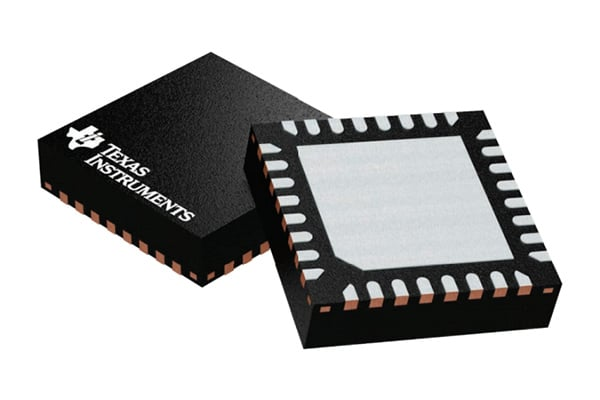
\includegraphics[width=0.5\textwidth]{figures/2_HW_figures/cc2640r2f.jpg}
    \caption{CC2640R2FRHB microcontroller.}
    \label{fig:cc2640r2f}
\end{figure}

According to the requirement ~\ref{req:mcu}, the Texas Instruments CC2640R2F was selected as the main microcontroller for the system. This device belongs to the SimpleLink family and features a 32-bit ARM Cortex-M3 core running at up to 48 MHz, 128 KB of flash memory, and 28 KB of RAM ~\cite{mcu_datasheet}. It also integrates a Bluetooth Low Energy (BLE) radio compliant with Bluetooth 5.1, which enables wireless communication with the mobile application. This MCu comes in three different package options: a 7x7 mm 48-pin VQFN package, a 5x5 mm 32-pin VQFN package, and a 4x4 mm 32-pin VQFN package. Considering the estimated GPIO usage of the system (see Table~\ref{tab:gpio_summary}), both 32-pin variants (including power and auxiliary pins) provide a sufficient number of I/O pins for the current architecture. The CC2640R2FRHB 5x5 mm package version was selected as it also provides a larger footprint compared with the 4x4 mm variant, making it more suitable for manual assembly.

\begin{table}[H]
\centering
\caption{Preliminary estimation on GPIO usage based on System Architecture}
\label{tab:gpio_summary}

\renewcommand{\arraystretch}{1.3}
\renewcommand{\tabularxcolumn}[1]{m{#1}}

\begin{tabularx}{\textwidth}{>{\raggedright\arraybackslash}X>{\centering\arraybackslash}c>{\raggedright\arraybackslash}X}
\toprule
\textbf{Subsystem} & \textbf{GPIO Usage} & \textbf{Interface Notes} \\
\midrule

Electrical Measurement Interface &
2-6 &
Serial interface (UART/I2C/SPI) + alert lines \\

Temperature Measurement &
1 &
Analog sensor connected to ADC pin \\

Display (User Interface) &
2-4 &
Serial interface (UART/I2C/SPI) possibly shared with electrical measurement \\

User Input &
1 &
Physical button with interrupt-capable GPIO \\

RF Communication (BLE) &
2-3 &
Integrated CC2640R2F BLE controller \\

Debug / Programming (JTAG) &
4 &
Standard JTAG interface (TMS, TCK, TDI, TDO, RESET) \\

\midrule
\textbf{Total Estimated GPIO Usage} &
\textbf{12-19 GPIOs} & \\
\bottomrule
\end{tabularx}
\end{table}

To allow proper operation of the MCU, as well as compliance with the system requirements, the following external components have been included within the MCU domain. In addition to the circuitry strictly required for microcontroller operation, this section also includes auxiliary components directly interfaced with the MCU and contributing to system-level functionalities.

\begin{itemize}
    \item \textbf{Reset Circuitry:} A low side push button combined with a \SI{100}{\kilo\ohm} pull-up resistor is connected to the RESET pin of the MCU to ensure it remains in a known state during power-up while also allowing manual reset during development and debugging activities. A \SI{100}{\nano\farad} capacitor is also included to improve reset signal stability, avoiding reset glitches. Since the push button is intended for development purposes, it will not be included in the final product.

    \item \textbf{Quartz Crystals:} A 24 MHz crystal oscillator is included as the main system clock source for the MCU, providing the required frequency stability for full-speed operation, peripheral timing, and communication interfaces.
    
    A dedicated 32.768 kHz crystal oscillator is included as a stable and low-drift reference clock for low-power modes and BLE sleep scheduling, ensuring compliance with the BLE timing requirements. In BLE connected operation, both master and slave devices are required to maintain a sleep clock accuracy within approximately ±500 ppm in order to guarantee correct timing of connection events and to limit the duration of the RX receive window. A less accurate sleep clock would increase the required guard time during reception windows, directly increasing average current consumption and reducing overall power efficiency.

    \item \textbf{Programming Interface:} A 4x2-pins JTAG header is provided for programming and debugging the MCU. This includes connections for TMS, TCK, TDI, TDO, and RESET signals, as well as VDD and GND pins connected according to Table ~\ref{tab:jtag_pinout}.
    
            \begin{table}[H]
                \centering
                \caption{4×2 JTAG Connector Pinout}
                \label{tab:jtag_pinout}

                \renewcommand{\arraystretch}{1.3}

                \begin{tabular}{r|c|c|l}
                    \cline{2-3}

                    GND  & 1 & 2 & TDI \\
                    \cline{2-3}

                    GND  & 3 & 4 & TDO \\
                    \cline{2-3}

                    NRESET  & 5 & 6 & TMSC \\
                    \cline{2-3}

                    VDD  & 7 & 8 & TCKC \\

                    \cline{2-3}

                \end{tabular}
            \end{table}
    \item \textbf{User Input Push Button}
        A low side push button, combined with a \SI{10}{\kilo\ohm} pull-up resistor, is connected to a GPIO pin of the MCU configured as an interrupt input, allowing the system to detect user actions without continuous polling. This button enables user interaction with the device, allowing display activation and the navigation between different screen views. A through-hole (TH) component has been selected beacause, in the final product, this interface represents the primary user interaction element and the TH implementation offers higher mechanical robustness and long-term reliability compared to smaller SMD alternatives. Moreover, during the development and testing phase, the system is operated without a mechanical enclosure, meaning that a standard surface-mounted tactile switch would be less comfortable to use and more exposed to mechanical damage.
    
    \item \textbf{Internal Power Supply Circuitry:}

        The CC2640R2F power architecture is based on three main internal supply domains: VDDS, VDDR, and VDDC. The VDDS rail represents the external supply input to the device and can operate over a wide voltage range. It feeds the internal power management unit, which generates all other required supply rails. The VDDR rail is the main regulated supply domain of the device and can be both generated internally or provided externally. It provides power to the RF subsystem and most internal functional blocks of the microcontroller. The VDDC rail is generated starting from the VDDS rail and is the supply rail that powers the digital logic and core of the MCU as well as the Always ON (AON) domain.   
            
        \begin{figure}[H]
            \centering
            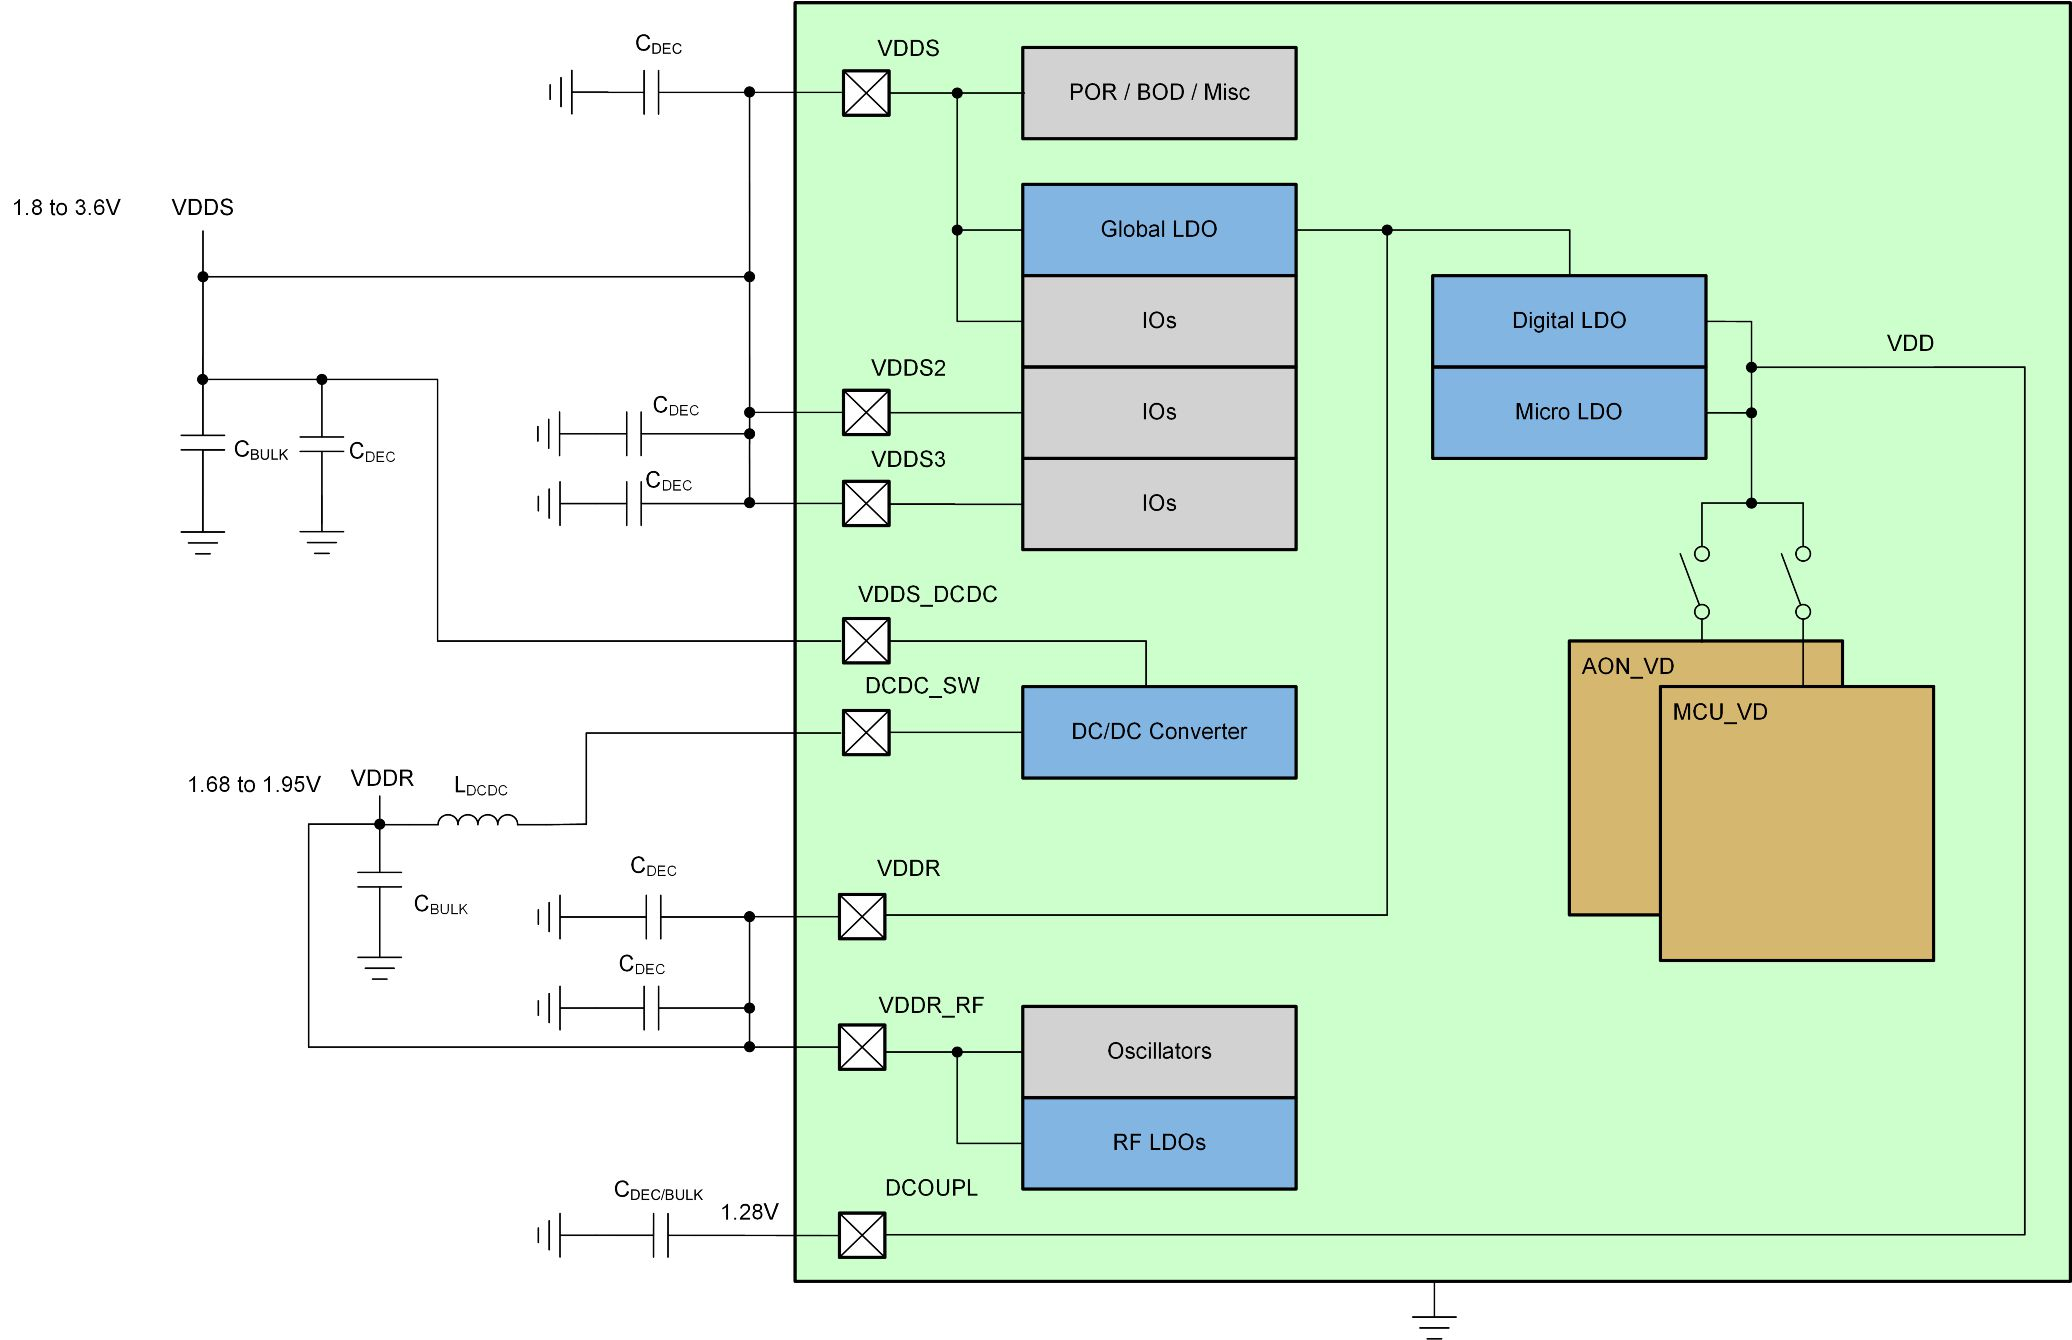
\includegraphics[width=0.85\textwidth]{figures/2_HW_figures/dcdc_converter_mode.jpg}
            \caption{CC2640R2F power architecture and supply configuration highlighting DC-DC converter operation mode.}
            \label{fig:cc2640_power_arch}
        \end{figure}

        The MCU supports three possible power supply configurations for the generation of the VDDR rail:

        \begin{itemize}
            \item \textbf{DC-DC Converter Mode:} The internal switching DC-DC converter generates VDDR from VDDS using an external inductor and capacitor. This mode provides high conversion efficiency and dynamically adapts to load conditions. When operating in this mode the VDDR rail source can be dinamically switched between the internal DC-DC converter and the internal Global LDO regulator, allowing the system to optimize power efficiency across different operating modes.

            \item \textbf{Global LDO Mode:} The VDDR rail is generated using only the internal LDO regulator. This configuration reduces external component count but results in overall higher power dissipation compared to DC-DC operation.

            \item \textbf{External Regulator Mode:} Both VDDS and VDDR are supplied externally, while the internal switching regulator and the Global LDO regulators are disabled. This mode is used when a dedicated external power management solution is available.
        \end{itemize}

        Among these configurations, DC-DC converter mode has been selected for this design.

        The primary reason for this choice is efficiency optimization. Since WattMate is a battery-powered and continuously operating measurement system, minimizing internal power consumption is critical to maximize operational lifetime. DC-DC operation allows the system to maintain higher efficiency across varying load conditions, which is particularly important during active measurement, BLE transmission and data display phases. Although it requires additional external components and careful PCB layout, this trade-off is justified by the substantial improvement in overall power efficiency and battery life.

        In addition, decoupling capacitors were added to ensure stable operation of the power supply rails, consisting of \SI{100}{\nano\farad} capacitors placed on all supply pins and one \SI{10}{\micro\farad} bulk capacitor on each of the main power rails.

\end{itemize}

%========================================================
% RF Antenna - Inverted-F Antenna
%========================================================
\newpage
\subsection{RF Antenna - Inverted-F Antenna}

The antenna selection process was guided by the aim of obtaining a compact solution, compliant with Bluetooth Low Energy (BLE) communication in the 2.4 GHz ISM band as required by \ref{req:ble_tx}. Among the various antenna technologies that still provide compact solutions, PCB-integrated antennas were preferred over chip antennas due to their lower cost and better RF performance, despite the increased occupied area. Based on the analysis of the Ti Antenna Selection Quick Guide~\cite{rf_quick_dn}, there main antenna alternatives were identified among pcb integrated antenna solutions: the Meandered Inverted F Antenna (MIFA), the Inverted F Antenna (IFA) and the Meandered Monopole Antenna. These three solutions were compared in terms of RF performance and occupied area, as summarized in Table~\ref{tab:pcb_antennas}.


\begin{table}[h]
\centering
\renewcommand{\arraystretch}{1.5}
\renewcommand{\tabularxcolumn}[1]{m{#1}}
\setlength{\tabcolsep}{6pt}

\caption{Comparison of different PCB antenna solutions}
\label{tab:pcb_antennas}

\begin{tabularx}{\textwidth}{>{\raggedright\arraybackslash}X>{\centering\arraybackslash}X>{\centering\arraybackslash}X>{\centering\arraybackslash}X}
\hline

\textbf{Antenna Type} &
Meandered Inverted F Antenna (MIFA) &
Inverted F Antenna (IFA) &
Meandered Monopole Antenna \\
\hline

\textbf{Layout Shape} &

\includegraphics[width=0.22\textwidth]{figures/2_HW_figures/mifa_antenna.jpg} &

\includegraphics[width=0.22\textwidth]{figures/2_HW_figures/ifa_antenna.jpg} &
\rule{0pt}{13ex}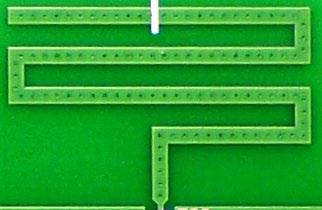
\includegraphics[width=0.18\textwidth]{figures/2_HW_figures/mono_antenna.jpg} \\
\hline

\textbf{Frequency} &
\SI{2.4}{\giga\hertz} &
\SI{2.4}{\giga\hertz} &
\SI{863}{\mega\hertz} + \SI{2.4}{\giga\hertz} (dual band) \\
\hline

\textbf{Typical Efficiency} &
68\% &
80\% &
94\% \\
\hline

\textbf{Bandwidth @ VSWR 2:0} &
\SI{101}{\mega\hertz} &
\SI{280}{\mega\hertz} &
\SI{354}{\mega\hertz} \\
\hline

\textbf{Dimensions (mm)} &
15 x 6 &
26 x 8 &
38 x 25 \\
\hline

\end{tabularx}

\end{table}

The IFA antenna was selected for this design because it provides a good trade-off between efficiency, bandwidth and occupied area. Thanks to its rectangular layout (width: 8mm similar to the MIFA) it can be easily integrated on one side of the PCB, allowing good RF domain separation while having minimal impact over the overall board geometry. Although the MIFA antenna provides a smaller footprint, its reduced efficiency and bandwidth compared to the IFA solution make it less suitable for this application, where reliability and ease of testing and debugging are key requirements. The meandered monopole antenna, while offering the best RF performance, was discarded due to its significantly larger dimensions. In Figure~\ref{fig:ifa_layout} is shown the implemented IFA layout, based on the TI application note~\cite{rf_ifa_ar} whose dimensions are shown in Table~\ref{tab:ifa_dimensions} for complenìteness.

\begin{figure}[H]
    \centering
    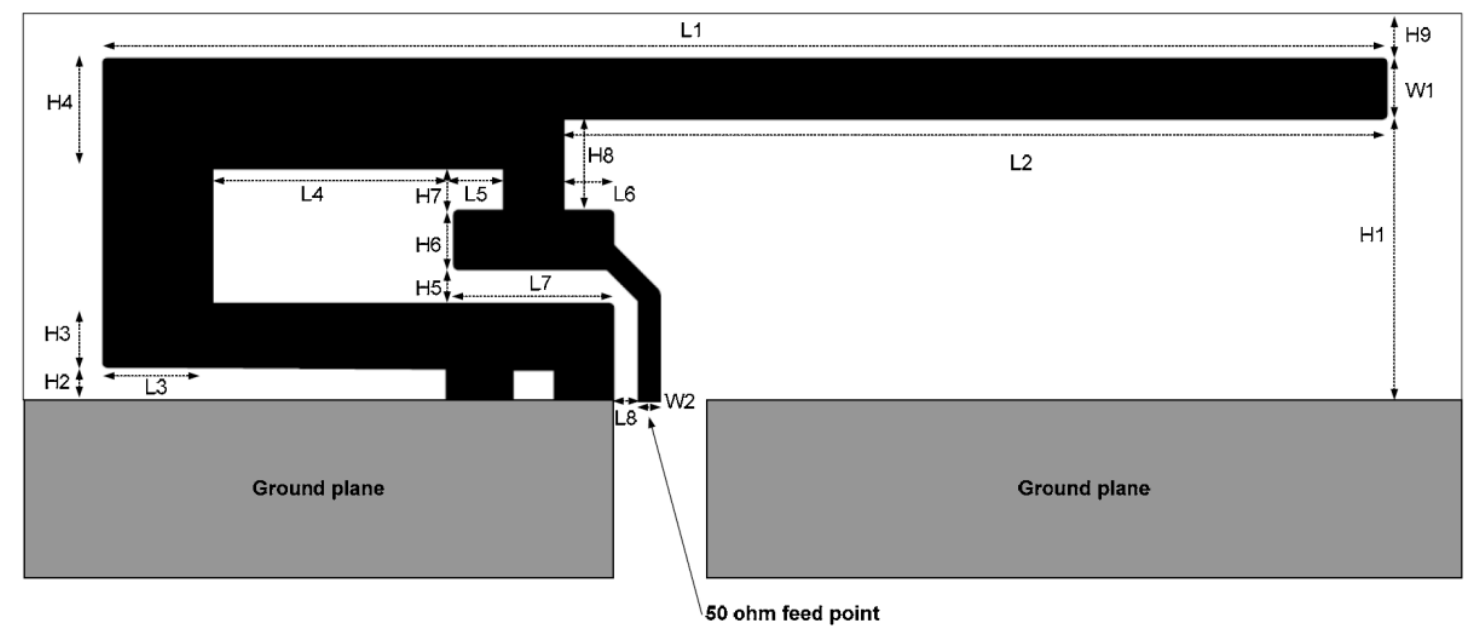
\includegraphics[width=0.95\textwidth]{figures/2_HW_figures/ifa_layout.png}
    \caption{Layout of the implemented Inverted F Antenna (IFA) solution.}
    \label{fig:ifa_layout}
\end{figure}

\begin{table}[h]
    \centering
    \caption{IFA Dimensions}
    \label{tab:ifa_dimensions}
    \renewcommand{\arraystretch}{1.3}

    \begin{tabularx}{\textwidth}{|>{\centering\arraybackslash}X|>{\centering\arraybackslash}X|>{\centering\arraybackslash}X|>{\centering\arraybackslash}X|}
        \hline
        \textbf{Parameter} & \textbf{Value} & \textbf{Parameter} & \textbf{Value} \\
        \hline
        H1 & 5.70 mm & W2 & 0.46 mm \\
        \hline
        H2 & 0.74 mm & L1 & 25.58 mm \\
        \hline
        H3 & 1.29 mm & L2 & 16.40 mm \\
        \hline
        H4 & 2.21 mm & L3 & 2.18 mm \\
        \hline
        H5 & 0.66 mm & L4 & 4.80 mm \\
        \hline
        H6 & 1.21 mm & L5 & 1.00 mm \\
        \hline
        H7 & 0.80 mm & L6 & 1.00 mm \\
        \hline
        H8 & 1.80 mm & L7 & 3.20 mm \\
        \hline
        H9 & 0.61 mm & L8 & 0.45 mm \\
        \hline
        W1 & 1.21 mm &  &  \\
        \hline
    \end{tabularx}
\end{table}

After selecting the appropriate \SI{2.4}{\giga\hertz} antenna solution, the RF front-end design was completed based on the comparison data provided in the application note~\cite{mcu_an}. The CC2640R2F supports four different RF front-end configurations , obtained through different combinations of signaling scheme and biasing options (see Figure~\ref{fig:rf_frontend}). The selected configuration for this design is the single-ended signaling scheme with external biasing. Single-ended signaling is preferred in applications where power consumption is a significant design constraint, while external biasing is used to maintain good sensitivity. The implemented front-end circuit is shown in Figure~\ref{fig:rf_frontend_circuit} and follows the reference design provided by Texas Instruments for single-ended implementation~\cite{rf_ifa_rd}.


\begin{figure}[H]
    \centering
    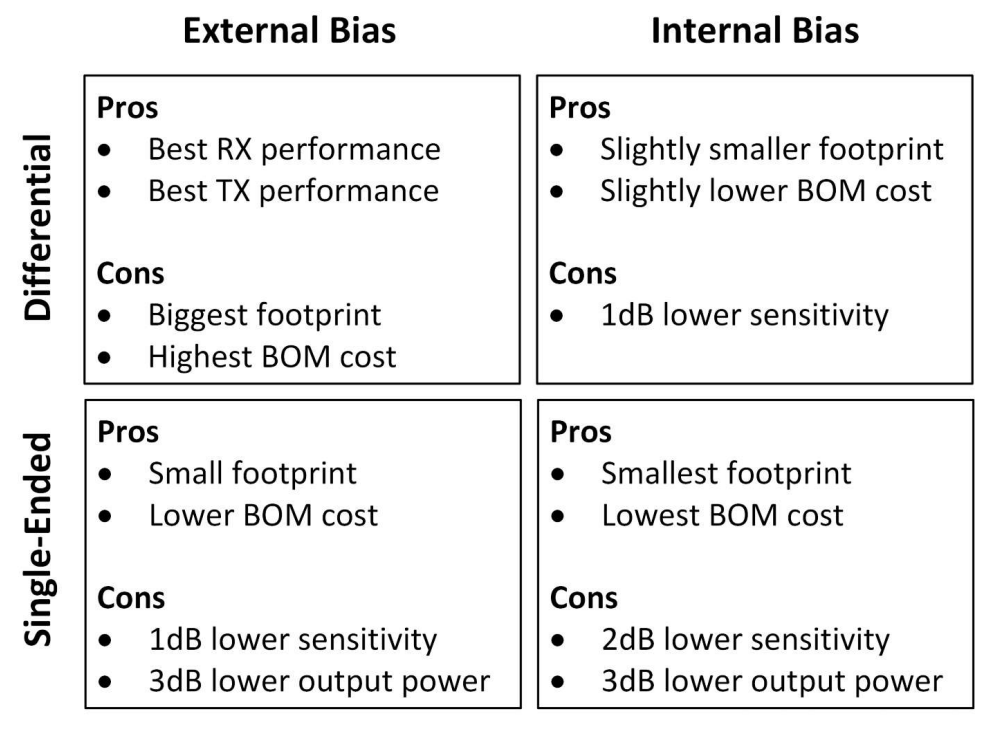
\includegraphics[width=0.7\textwidth]{figures/2_HW_figures/rf_front_end.png}
    \caption{Comparison of CC13xx/CC26xx Front-End Configuration.}
    \label{fig:rf_frontend}
\end{figure}

\begin{figure}[H]
    \centering
    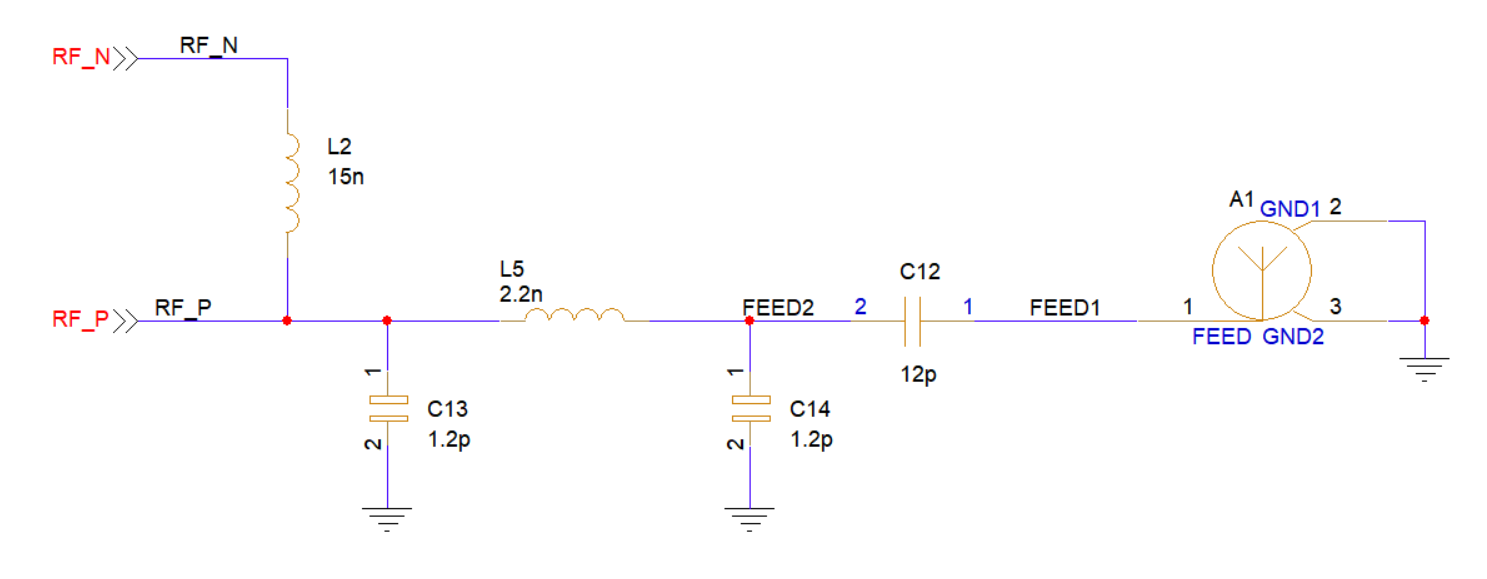
\includegraphics[width=1\textwidth]{figures/2_HW_figures/rf_frontend_circuit.png}
    \caption{Implemented RF Front-End circuit.}
    \label{fig:rf_frontend_circuit}
\end{figure}


%========================================================
% Voltage and Current Sensor - PAC1951
%========================================================
\newpage
\subsection{Voltage and Current Sensor - PAC1951}

\subsubsection{Uncertainty Analysis}
The current measurement sensing architecture is based on a precision shunt resistor $R_S$, where the load current is indirectly obtained from the voltage drop across it. Among the possible sensor technologies, the preferred solution is the use of a dedicate current and voltage measurement IC, which internally integrates the ADC and provide a digital output to the MCU. This approach was selected over discrete implementations based on operational amplifiers and MCU internal ADCs because it allows the MCU to remain in low-power modes during measurement aquisition. For the chosen architecture the nominal current measurement is given by:

\begin{equation}\label{current_meas}
I_S = \frac{V_{S}}{R_S}
\end{equation}

However, the actual measurement is affected by two independent error sources:
\begin{itemize}
    \item \textbf{ADC Measurement Uncertainty:} The internal ADC of the PAC1951 introduces gain error, offset error and integral non-linearity that affect the accuracy of the voltage measurement across the shunt resistor.
    According to the standard ADC error model, the total measurement uncertainty can be expressed as:

    \begin{equation}\label{adc_error}
        \Delta V_{S} = \Delta G \cdot V_{S} + INL \cdot V_{S} + V_{OFF} + \frac{Q}{2}
    \end{equation}

    where:
    \begin{itemize}
        \item $V_{S}$ is the voltage drop across the shunt resistor,
        \item $\Delta G$ is the gain error of the measurement system,
        \item $INL$ is the integral non-linearity of the ADC,
        \item $V_{OFF}$ is the input-referred offset voltage of the ADC,
        \item $Q$ is the quantization step of the ADC
    \end{itemize}
    
    \item \textbf{Shunt Resistor Tolerance:} The shunt resistor $R_S$ has a specified tolerance ($\Delta R_S$) that contributes to the overall measurement uncertainty.

\end{itemize}

Following a first-order uncertainty propagation approach, starting from Eq.~\ref{current_meas}, the total current measurement error can be expressed as:

\begin{equation}
\Delta I_S = \frac{\Delta V_{S} + \Delta R_{S} \cdot I_S}{R_S}
\end{equation}

from which the relative error expression is obtained by substituting Eq.~\ref{adc_error} for $\Delta V_{S}$:

\begin{equation}
\varepsilon_{rel} = \frac{\Delta I_{S}}{I_{S}} =
\Delta G + INL + \Delta R_S +
\frac{V_{OFF} + \frac{Q}{2}}{R_S \cdot I_S}
\end{equation}


The first three terms represent static gain and component-related uncertainties, while the last term introduces a current-dependent contribution that dominates at low current levels. This term explains the steep increase in relative error observed in the low-current region. This formulation was used to compare different current sensing solutions by evaluating their sensitivity to measurement uncertainty over the operating range defined by the requiremnt~\ref{req:measurement-current}.

Similarly to the current measurement, the nominal voltage measurement is given by:
\begin{equation}
V_{BUS} = V_{meas}
\end{equation}

The measurement is affected by the same ADC-related uncertainty sources described for the current channel, namely gain error, integral non-linearity, offset voltage, and quantization error. The total voltage uncertainty can be expressed as:

\begin{equation}\label{adc_v_uncertainty}
\Delta V_{BUS} =
\Delta G \cdot V_{BUS} +
INL \cdot V_{BUS} +
V_{OFF} + \frac{Q}{2}
\end{equation}

Unlike the current measurement, no shunt resistor contribution is present, so the uncertainty is dominated by ADC non-idealities and becomes less dependent on the measured value. This results in a more uniform relative error across the operating range.

\subsubsection{Sensor Selection}
\begin{figure}[H]
    \centering
    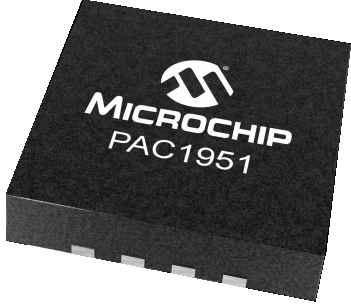
\includegraphics[width=0.35\textwidth]{figures/2_HW_figures/pac1951.png}
    \caption{PAC1951T-1E/4MX sensor.}
    \label{fig:pac1951}
\end{figure}

The PAC1951 was selected as the current and voltage monitoring IC because its characteristics closely match the measurement, power consumption, and system integration requirements defined for WattMate. The most relevant features that motivated this choice are summarized below:

\begin{itemize}

    \item \textbf{Electrical Characteristics:}

    \begin{table}[H]
        \centering
        \renewcommand{\arraystretch}{1.3}
        \caption{Electrical characteristics of the PAC1951 power monitor}
        \label{tab:pac1951_electrical}

        \begin{tabularx}{0.9\textwidth}{|l|X|c|c|c|}
            \hline
            \textbf{Symbol} &
            \textbf{Parameters} &
            \textbf{Typical} &
            \textbf{Maximum} &
            \textbf{Unit} \\
            \hline

            $V_{DD}$ & Supply voltage & 3.3 & 5.5 & \SI{}{\volt} \\
            \hline

            \multirow{2}{*}{$I_{DD,ACTIVE}$} 
            & Active supply current (1024 SPS) & 395 & 535 & \SI{}{\micro\ampere} \\ \cline{2-5}
            & Active supply current (8 SPS) & 12 & 130 & \SI{}{\micro\ampere} \\
            \hline

            $I_{DD,SLEEP}$ & Sleep mode supply current & 5 & - & \SI{}{\micro\ampere} \\
            \hline

        \end{tabularx}
    \end{table}
    The PAC1951 requires a low-voltage supply rail, $V_{DD}$, to power its internal digital logic and I\textsuperscript{2}C interface. The same $V_{DD}$ power rail is also used to supply the analog section of the current and voltage sensing circuitry within the IC.

    \item \textbf{Bus Voltage Measurement Range:}  
    The device supports bus voltage measurements from \SI{0}{\volt} to \SI{32}{\volt}, satisfying the operating voltage requirements up to the \SI{28}{\volt} USB Power Delivery profile defined in Requirements~\ref{req:volt_nominal} and ~\ref{req:volt_rating}.

    \item \textbf{Bidirectional Current Measurement:}  
    The PAC1951 supports bidirectional current sensing through differential shunt voltage measurement with full-scale ranges up to $\pm\SI{100}{\milli\volt}$ that can be programmed dynamically via the control registers to optimize measurement resolution for different load conditions. Combined with a \SI{10}{\milli\ohm} shunt resistor value, this allows accurate measurement of charge and discharge currents up to $\pm\SI{10}{\ampere}$, complying with Requirement~\ref{req:curr_rating}.

    \item \textbf{High Measurement Resolution and Accuracy:}  
    By substituting the worst-case non-ideality parameters reported in the PAC1951 datasheet~\cite{pac1951_datasheet} into the previously derived error model equations, it can be shown that the selected sensor is capable of achieving better than \SI{0.5}{\percent} voltage measurement accuracy and better than \SI{1}{\percent} current measurement accuracy across the specified operating range. This result can be achievd thanks the 16-bit ADCs resolution and the real-time auto-calibration of voltage and current offset error provided by the PC1951.
    Voltage and current error curves were obtained on the entire operating range to verify the compliance with the accuracy requirements, as shown in Figure~\ref{fig:pac1951_error_curves}. Although these values are derived considering worst-case datasheet parameters, the obtained performance still satisfies the requirements defined in~\ref{req:volt_acc} and~\ref{req:curr_acc}. 

    \begin{figure}[H]
        \centering
        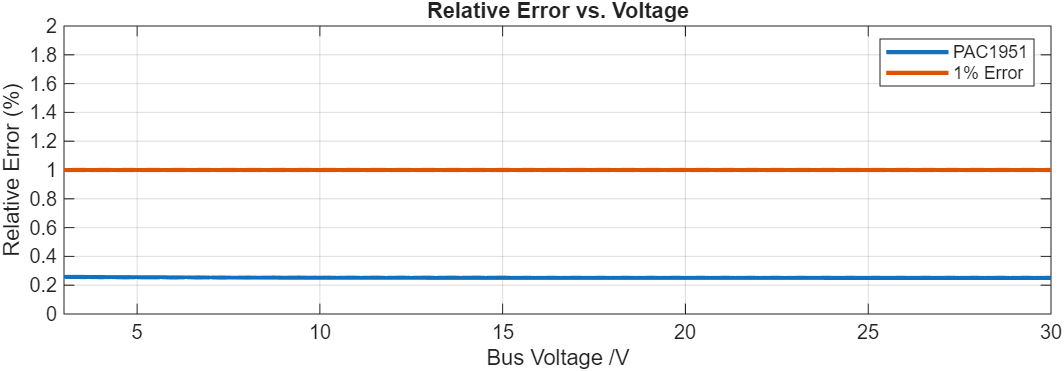
\includegraphics[width=0.8\textwidth]{figures/2_HW_figures/pac_volt_uncertainty.png}
        \vspace{0.5cm}

        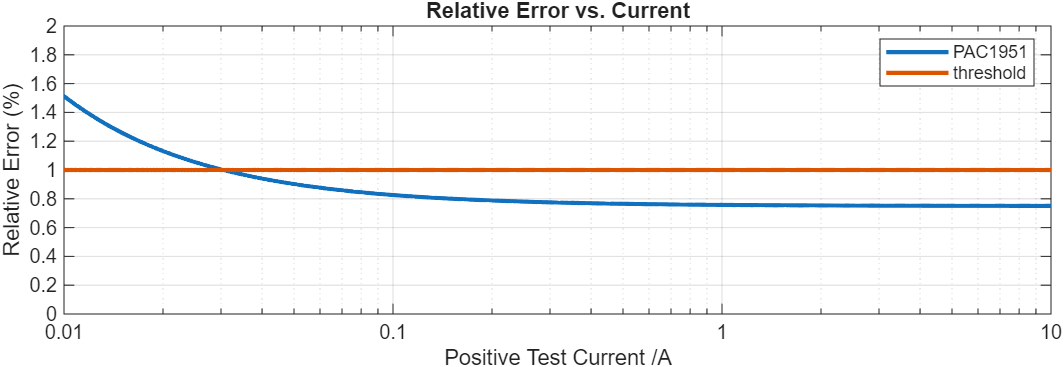
\includegraphics[width=0.8\textwidth]{figures/2_HW_figures/pac_curr_uncertainty.png}
        \caption{Worst case voltage and current measurement error curves for the PAC1951.}
        \label{fig:pac1951_error_curves}
    \end{figure}

    Additionally, given the uncertainty values obtained for voltage and current measurements, the resulting power measurement uncertainty is less than \SI{2}{\percent}, verifying compliance with Requirement~\ref{req:pow_acc}.

    \item \textbf{Integrated Power and Energy Computation:}  
    The PAC1951 internally performs power computation and energy accumulation using dedicated hardware registers. This reduces MCU computational load while supporting the derived quantity calculations required by Requirement~\ref{req:data_proc}.

    \item \textbf{Programmable Sampling Rate:}  
    The device supports programmable sampling rates from \SI{8}{\second\per\second} to \SI{1024}{\second\per\second}, enabling the implementation of different acquisition strategies according to the required measurement update frequency. These capabilities largely exceed the minimum acquisition frequency required by Requirement~\ref{req:perf_sampling}, providing additional design margin.

    \item \textbf{Low-Power System Compatibility:}  
    Since the PAC1951 autonomously performs measurements and accumulation, the MCU can remain in low-power operating modes between acquisitions. This characteristic contributes to compliance with the low-power requirements~\ref{req:pwr_consumption} and~\ref{req:pwr_battery}. Furthermore, when no significant power flow is detected, the PAC1951 can be configured to operate at the minimum sampling rate of \SI{8}{\second^{-1}}, reducing its supply current to \SI{12}{\micro\ampere}, providing additional power saving opportunity.

    \item \textbf{Integrated Fault Detection and ALERT Outputs:}  
    The PAC1951 includes programmable over-voltage, under-voltage, over-current, and overpower detection features, together with two configurable open-drain ALERT outputs. These outputs are connected to MCU interrupt inputs through pull-up resistors, allowing fault conditions to immediately notify the MCU or wake it from low-power modes when an abnormal operating condition is detected.These features simplify the implementation of the protection and notification mechanisms required by Requirements~\ref{req:over_alert} and~\ref{req:under_alert}.

    \item \textbf{Digital I\textsuperscript{2}C Interface:}  
    Communication with the MCU is performed through a standard I\textsuperscript{2}C interface, simplifying PCB routing and reducing the number of required MCU peripherals.

    \item \textbf{Package:}  
    The PAC1951 is available in both 16-pin 3 x 3 mm VQFN and 16-pin 2.2 x 2.2 mm WLCSP packages. The PAC1951T-1E/4MX 3 x 3 mm VQFN package version was selected for this design, as it provides a good balance between compactness and ease of manual assembly, improving manufacturability according to Requirement~\ref{req:assembly}.

\end{itemize}

\begin{figure}[H]
    \centering
    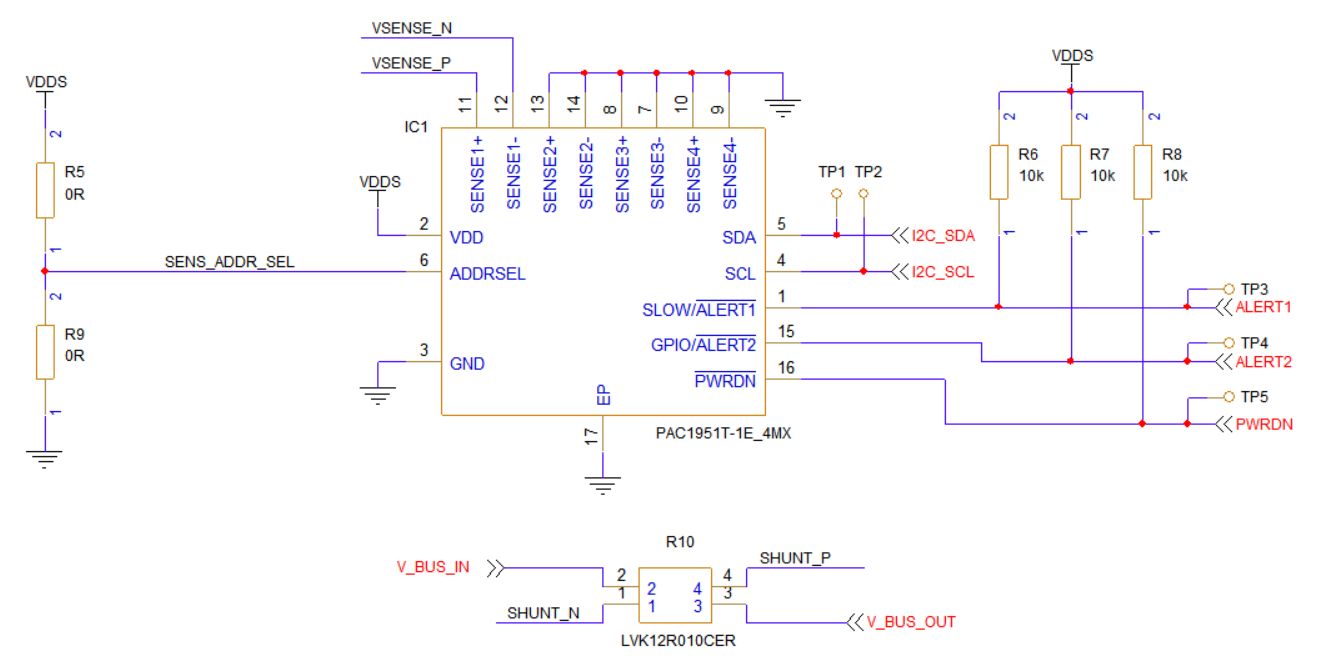
\includegraphics[width=0.95\textwidth]{figures/2_HW_figures/pac_circuit.png}
    \caption{Implemented PAC1951 sensing circuit.}
    \label{fig:pac_circuit}
\end{figure}

To achieve the error performance shown in Figure~\ref{fig:pac1951_error_curves}, a precision shunt resistor is required. In this design, a \SI{10}{\milli\ohm} resistor with \SI{0.25}{\percent} tolerance was selected. The chosen component features dedicated Kelvin sense terminals, which are exclusively used for routing the voltage sensing signals. This configuration improves measurement accuracy by minimizing the impact of parasitic voltage drops along the high-current path and reducing susceptibility to noise.

To further provide noise filtering capability, a differential low-pass input filter was placed between the shunt resistor and the PAC1951 sensing inputs, as shown in Figure~\ref{fig:pac1951_input_filter}. The filter was included as a design margin to allow additional noise mitigation if excessive interference from the environment, switching regulators, or other high-frequency sources is observed during the validation phase. The filter is implemented symmetrically on both sensing lines to preserve differential measurement accuracy and maintain common-mode noise rejection.

Under normal operating conditions, the PAC1951 does not require external input filtering thanks to its internal architecture and real-time offset calibration. However, following discussions with the device vendor, space for a differential input filter was reserved on the PCB to allow future noise mitigation measures, if required, without the need for hardware redesign. 

\begin{figure}[H]
    \centering
    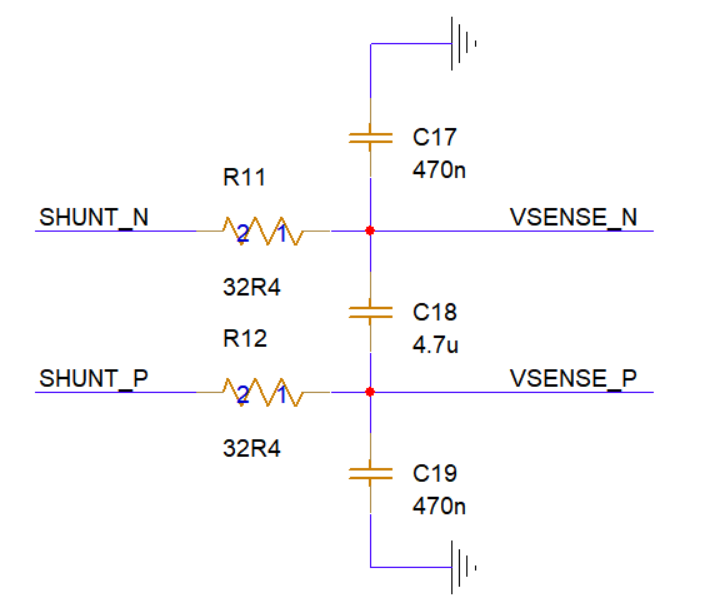
\includegraphics[width=0.55\textwidth]{figures/2_HW_figures/pac1951_input_filter.png}
    \caption{Differential low-pass filter placed between the shunt resistor and the PAC1951 sensing inputs.}
    \label{fig:pac1951_input_filter}
\end{figure}

%========================================================
% Temperature Sensor - NTC Thermistor
%========================================================
\newpage
\subsection{Temperature Sensor - NTC Thermistor}\label{ntc}

The proposed temperature sensing topology is based on a Negative Temperature Coefficient (NTC) thermistor configured in a resistive voltage divider. This sensing approach has been selected as it provides a simple, low-cost and low-power solution for temperature acquisition while maintaining compliance with the system requirements defined in~\ref{req:measurement-temperature}, which are not sufficiently stringent to justify higher-precision and higher-cost sensing solutions. In addition, the use of a thermistor enables a highly flexible placement strategy, which is essential to support the monitoring of the external battery pack, by choosing a leaded package (an approach that would not be easily achievable with integrated IC temperature sensors). The proposed sensing circuit (see Figure~\ref{fig:ntc_divider_circuit}) implement a direct connection with the MCU ADC, avoiding the need for additional digital communication interfaces and simplifying system integration.

\begin{figure}[H]
    \centering
    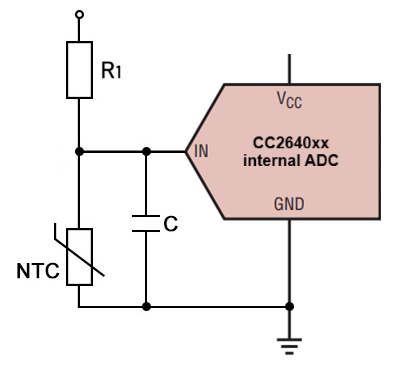
\includegraphics[width=0.4\textwidth]{figures/2_HW_figures/ntc_arch.png}
    \caption{NTC temperature sensing circuit based on a resistive voltage divider.}
    \label{fig:ntc_divider_circuit}
\end{figure}


\subsubsection{Uncertainty Analysis}

\begin{equation}
R_{NTC}(T) = R_0 \, \exp\left[\beta \left(\frac{1}{T} - \frac{1}{T_0}\right)\right]
\end{equation}

where $R_0$ is the nominal resistance at reference temperature $T_0 = \SI{25}{\celsius}$ and $\beta$ is the material constant of the thermistor.
By measuring the output voltage $V_O$ of the resistive divider, the resistance of the thermistor can be expressed as:

\begin{equation}\label{res_div}
R_{NTC} = R_1 \frac{V_O}{V_{DD} - V_O}
\end{equation}

Temperature is then recovered by inverting the Beta equation:

\begin{equation}\label{temp_meas}
T = \left[\frac{1}{T_0} + \frac{1}{\beta}\ln\left(\frac{R_{NTC}}{R_0}\right)\right]^{-1}
\end{equation}


The temperature estimation uncertainty is obtained through first-order propagation applied to the nonlinear transformation. 

\begin{equation}
\label{eq:ntc_total_partial}
\Delta T =
\left|\frac{\partial T}{\partial \beta}\right|\Delta \beta +
\left|\frac{\partial T}{\partial R_0}\right|\Delta R_0 +
\left|\frac{\partial T}{\partial R_{NTC}}\right|\Delta R_{NTC}
\end{equation}


From~\ref{eq:ntc_total_partial}, it is clear that the total uncertainty is decomposed into independent contributions:

\begin{equation}
\Delta T = \Delta T_{\beta} + \Delta T_{R_0} + \Delta T_{R_{NTC}}
\end{equation}

\begin{itemize}

    \item \textbf{Beta parameter uncertainty}

        This term accounts for the sensitivity of the temperature estimation to variations in the thermistor $\beta$ parameter, which introduces a nonlinear error that increases with the logarithmic resistance ratio. By derivating Eq.~\ref{temp_meas} the beta parameter uncertainty term results:

        \begin{equation}
        \Delta T_{\beta} =
        \frac{1}{D^2}
        \left|\frac{\ln\left(\frac{R_{NTC}}{R_0}\right)}{\beta^2}\right|
        \Delta \beta
        \end{equation}

        with

        \begin{equation}
        D = \frac{1}{T_0} + \frac{1}{\beta}\ln\left(\frac{R_{NTC}}{R_0}\right)
        \end{equation}

    
    \item \textbf{Nominal resistance tolerance}
    
    This term represents the effect of the tolerance of the nominal resistance $R_0$ on the temperature estimation accuracy, acting as a constant scaling uncertainty over the full operating range.
        \begin{equation}
        \Delta T_{R_0} =
        \frac{1}{D^2}
        \left|\frac{1}{\beta R_0}\right|
        \Delta R_0
        \end{equation}

\item \textbf{Measured resistance contribution}

The resistance is measured indirectly by knowing the value of the resistor $R_1$ in the voltage divider and by measuring the output voltage of the divider. This approach introduces two additional sources of uncertainty: the error on the measured voltage, due to the ADC, and the tolerance of the resistor $R_1$. By introducing the resistive divider relationship of Eq.~\ref{res_div}, the voltage-related uncertainty propagates to the temperature estimation as follows:

\begin{equation}
\Delta T_{V_O} =
\frac{1}{D^2}
\left|\frac{1}{\beta R_{NTC}}\right|
\left|\frac{R_1 V_{DD}}{(V_{DD} - V_O)^2}\right|
\Delta V_O
\end{equation}

The same reasoning can be applied on the temperature uncertainty term related to the tolerance of the $R_1$ resistor, obtaining:

\begin{equation}
\Delta T_{R_1} =
\frac{1}{D^2}
\left|\frac{1}{\beta R_{NTC}}\right|
\left|\frac{V_O}{V_{DD} - V_O}\right|
\Delta R_1
\end{equation}

\end{itemize}


The total temperature measurement uncertainty is therefore:

\begin{equation}
\Delta T =
\Delta T_{\beta} + \Delta T_{R_0} + \Delta T_{V_O} + \Delta T_{R_1}
\end{equation}


\subsubsection{Sensor Selection}

\begin{figure}[H]
    \centering
    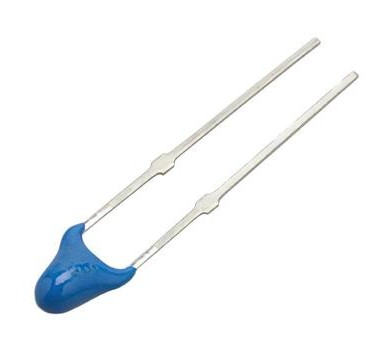
\includegraphics[width=0.35\textwidth]{figures/2_HW_figures/ntc.jpg}
    \caption{103AP-2 NTC sensor.}
    \label{fig:ntc}
\end{figure}

Based on the derived uncertainty model and on the resulting analysis, shown in Figure~\ref{fig:ntc_uncertainty}, the 103AP-2 NTC thermistor was selected in combination with a \SI{5.76}{\kilo\ohm}, \SI{0.1}{\percent} pull-up resistor. The most relevant features that motivated this choice are summarized below:

\begin{itemize}

    \item \textbf{Electrical and uncertainty-related parameters}

        The electrical parameters reported in Table~\ref{tab:ntc_103ap2_params} define both the nominal behavior of the thermistor and its associated modeling uncertainties. In particular, the tolerances on $R_0$ and $\beta$, together with the $R_1$ parameters,  directly affect the temperature estimation accuracy. The chosen combination of components allows compliancy with requirement~\ref{req:temp_acc} (see Figure~\ref{fig:ntc_uncertainty}).

        \begin{table}[H]
            \centering
            \renewcommand{\arraystretch}{1.3}
            \caption{Electrical and uncertainty parameters of the 103AP-2 NTC sencing circuit}
            \label{tab:ntc_103ap2_params}

            \begin{tabular}{|l|l|}
                \hline
                \textbf{Parameter} & \textbf{Value / Description} \\
                \hline
                Nominal resistance $R_0$ & $\SI{10}{\kilo\ohm}$ @ \SI{25}{\celsius} \\
                \hline
                Resistance tolerance & $\pm 0.5\%$ \\
                \hline
                Beta parameter $\beta$ & $\SI{3435}{\kelvin}$ \\
                \hline
                Beta parameter tolerance & $\pm 0.5\%$ \\
                \hline
                Pull-up resistor $R_1$ & $\SI{5.76}{\kilo\ohm}$ \\
                \hline
                Pull-up resistor tolerance & $\pm 0.1\%$ \\
                \hline
            \end{tabular}
        \end{table}

    \item \textbf{Mechanical and environmental characteristics}
        \begin{itemize}
            \item Operating temperature range: \SI{-60}{\celsius} to \SI{150}{\celsius}
            \item Leaded epoxy-coated package enabling flexible placement and off-board sensing
            \item Small sensing element enclosure enabling thermal rise constant of 15 seconds (when suspended in mid-air)
        \end{itemize}


\end{itemize}

\begin{figure}[H]
    \centering
    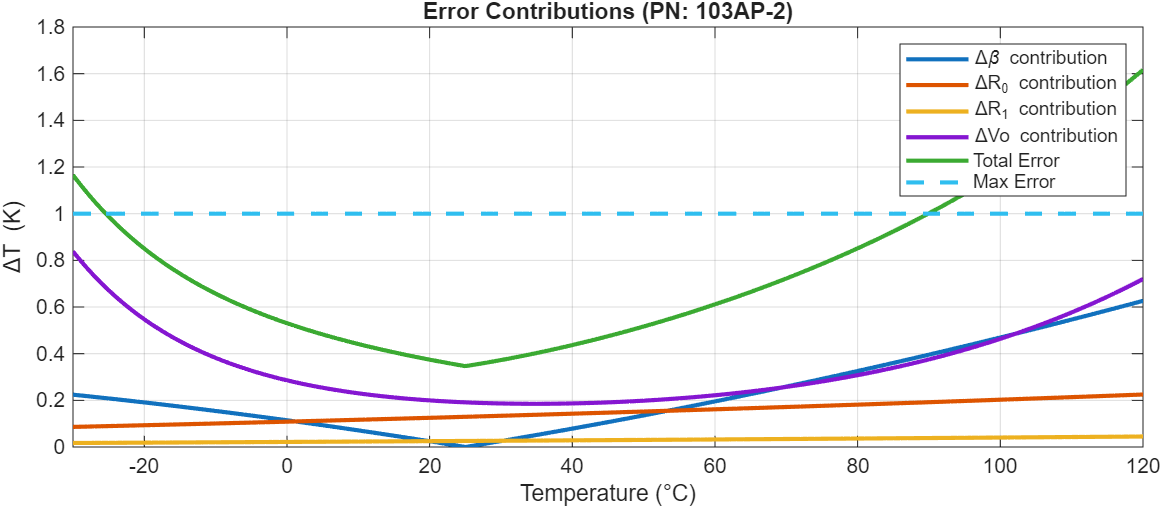
\includegraphics[width=0.9\textwidth]{figures/2_HW_figures/ntc_uncertainty.png}
    \caption{Temperature measurement uncertainty contributions for the selected NTC sensor.}
    \label{fig:ntc_uncertainty}
\end{figure}

Figure~\ref{fig:ntc_circuit} shows the actual implementation of the NTC sensing circuit. In addition to the previously described voltage divider topology, a high-side MOSFET $Q_1$ was introduced to enable the NTC sensing circuit only when temperature acquisition is required, making its leakage current contribution negligible during MCU low-power operation. The gate pull-up resistor $R_{13}$ ensures that the sensing branch is automatically disabled whenever the enable control signal is left floating or interrupted.

At room temperature, the voltage divider dissipates approximately \SI{0.69}{\milli\watt} during ON-state operation. If continuously powered, this static consumption would significantly impact the OFF-state efficiency and reduce the expected battery lifetime, conflicting with the low-power requirements defined in~\ref{req:pwr_battery} and~\ref{req:pwr_consumption}.

\begin{figure}[H]
    \centering
    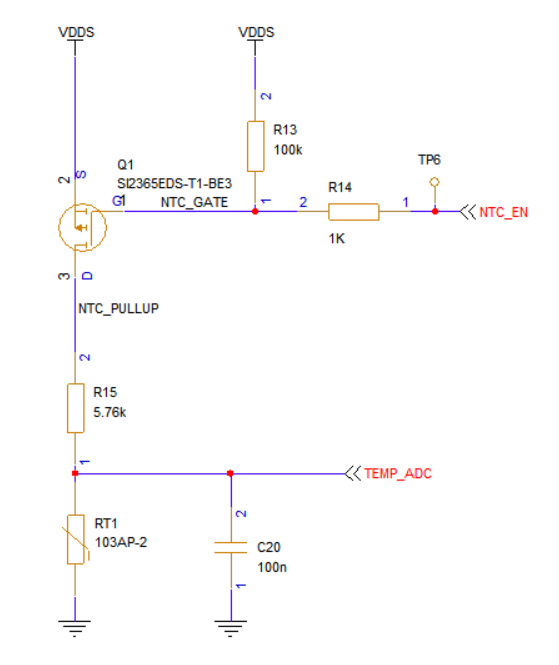
\includegraphics[width=0.55\textwidth]{figures/2_HW_figures/ntc_circuit.png}
    \caption{Implemented NTC sensing circuit with high side switch.}
    \label{fig:ntc_circuit}
\end{figure}


%========================================================
% Display - OLED Display
%========================================================
\newpage
\subsection{Display - OLED Display}

\begin{figure}[htbp]
    \centering
    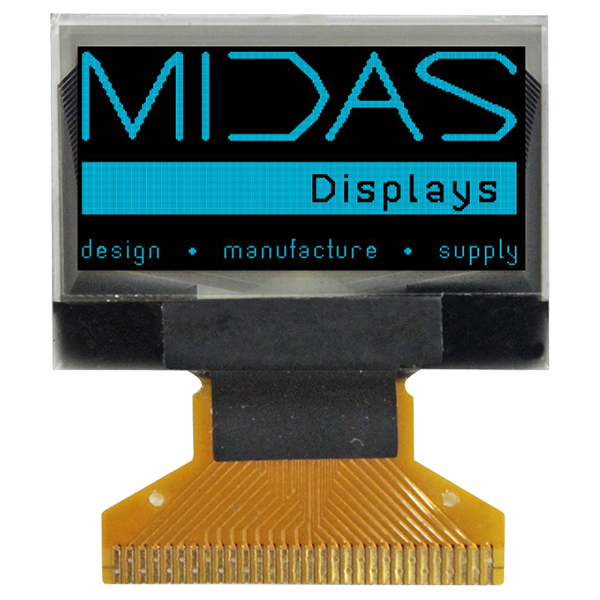
\includegraphics[width=0.4\textwidth]{figures/2_HW_figures/oled_display.png}
    \caption{MCOT128064N2Z-BM OLED display module.}
    \label{fig:oled_display}
\end{figure}

The integration of the OLED display enables the local visualization of measurements, directly satisfying Requirement~\ref{req:ui_display}. The selected display module is the MCOT128064N2Z-BM, a monochrome OLED display featuring a 0.96-inch active area and a resolution of 128 x 64 pixels. The most relevant features and implementation details that motivated this choice are summarized below:

\begin{itemize}

    \item \textbf{Integrated Controller}
    
    The display is based on the widely adopted SSD1306 display controller, which is directly embedded inside the module. This driver integrates both logic and power functionalities, reducing the need for external components and minimizing the overall footprint on the PCB.

    \item \textbf{Electrical Characteristics:}
    
    \begin{table}[H]
        \centering
        \renewcommand{\arraystretch}{1.3}
        \caption{Electrical characteristics of the MCOT128064N2Z-BM display module}
        \label{tab:oled_electrical}

        \begin{tabularx}{0.9\textwidth}{|l|X|c|c|c|}
            \hline
            \textbf{Symbol} &
            \textbf{Parameters} &
            \textbf{Typical} &
            \textbf{Maximum} &
            \textbf{Unit} \\
            \hline

            $V_{DD}$ & Logic supply voltage & 3.3 & 4.0 & \SI{}{\volt} \\
            \hline

            $I_{DD}$ & Normal operation, full display ON & 42 & 127 & \SI{}{\micro\ampere} \\
            \hline

            $I_{DD,SLEEP}$ & Display OFF & - & 10 & \SI{}{\micro\ampere} \\
            \hline

            $V_{CC}$ & Segment supply voltage generated by charge pump & 7.5 & - & \SI{}{\volt} \\
            \hline

            $I_{CC}$ & Normal operation, 50\% display ON & 25.6 & 32 & \SI{}{\milli\ampere} \\
            \hline

        \end{tabularx}
    \end{table}
    The SSD1306 controller requires a low-voltage supply rail, $V_{DD}$, to power its internal digital logic. In addition, the OLED panel requires a higher driving voltage, $V_{CC}$, to supply the display segments. Since the voltage required to drive the OLED pixels is significantly higher than the logic supply voltage, the controller internally generates $V_{CC}$ from the input supply through an integrated charge pump. This is implemented by connecting external \SI{1}{\micro\farad} flying capacitors across the C1P/C1N and C2P/C2N pins, allowing the controller to generate $V_{CC}$ directly from the supply voltage ($V_{DD}$).

    \item \textbf{Serial Interface:} 
    
    To minimize the number of required GPIO pins and simplify PCB routing, the display is configured for I\textsuperscript{2}C communication by connecting the interface configuration pins to the logic levels specified by the SSD1306 controller datasheet.

    \item \textbf{OLED Technology:} 
    
    Unlike traditional LCDs that require a constant power-drawing backlight, the OLED panel consumes power only for its active (lit) pixels. This significantly improves energy efficiency during ON-State operation, supporting Requirement~\ref{req:pwr_consumption}. Moreover, the absence of a backlighting system allows the display to be thinner compared to alternative technologies. Additionally, the OLED panel provides a high contrast ratio and a wide viewing angle to ensure excellent readability.

    \item \textbf{Hardware Contrast Calibration:} 
    
    The panel's brightness and maximum segment current ($I_{SEG}$) are hardware-calibrated via an internal reference current ($I_{REF}$). To achieve the recommended segment current of \SI{100}{\micro\ampere} at the maximum software contrast setting of 255, a precision external pull-down resistor is connected between the $I_{REF}$ pin and analog ground ($V_{SS}$). This maintains the reference current at exactly \SI{12.5}{\micro\ampere}.

    \item \textbf{Mechanical Mounting:} Thanks to the flexible cable, the display can be mounted on the opposite side of the PCB with respect to the connector location by folding the flex cable around the board edge. This approach minimizes the effective PCB footprint, as only the SMD connector occupies board space, while the display module itself is positioned outside the populated side of the PCB.

\end{itemize}



\begin{figure}[htbp]
    \centering
    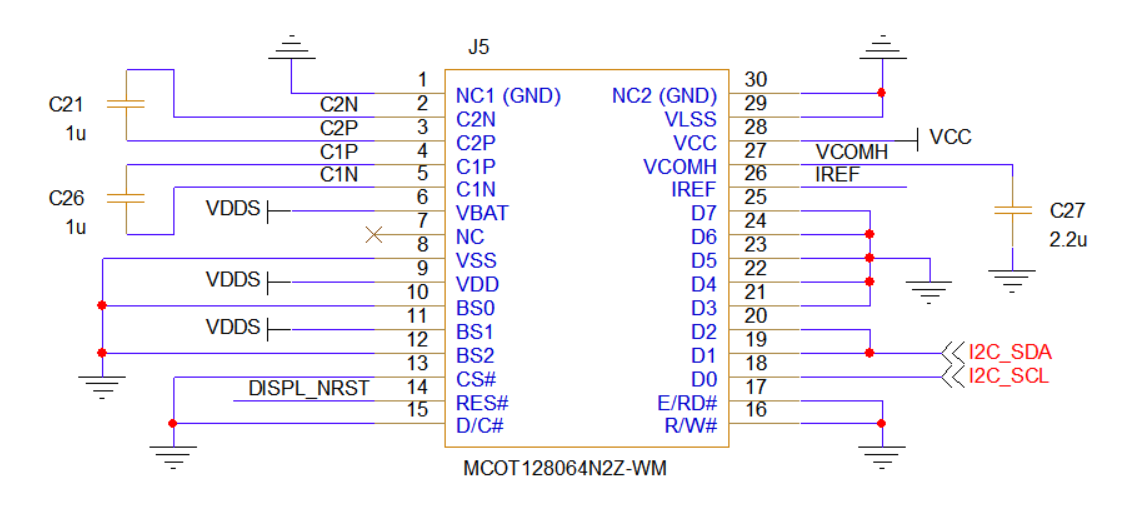
\includegraphics[width=0.9\textwidth]{figures/2_HW_figures/oled_circuit.png}
    \caption{Implemented OLED display circuit.}
    \label{fig:oled_schematic}
\end{figure}

%========================================================
% Power Supply - MAX77597
%========================================================
\newpage
\subsection{Power Supply - MAX77597}\label{sec:schematic_max77597}

\begin{figure}[H]
    \centering
    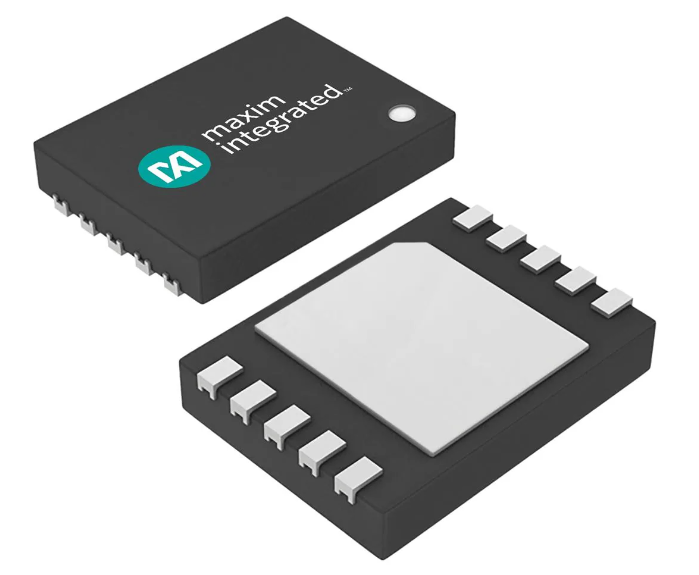
\includegraphics[width=0.4\textwidth]{figures/2_HW_figures/max77597.png}
    \caption{MAX77597ETBB+T synchronous buck converter controller.}
    \label{fig:dcdc}
\end{figure}

As shown in Table~\ref{tab:voltage_summary}, all the circuit subsystems were chosen to be powered by a stable \SI{3.3}{\volt} voltage rail. This rail must be derived directly from the power bus, which can range from \SI{5}{\volt} to \SI{28}{\volt} with a \SI{+5}{\percent} tolerance (up to \SI{29.4}{\volt}) as defined in Requirements~\ref{req:volt_nominal} and~\ref{req:volt_rating}. To fulfill this, the MAX77597 synchronous step-down converter was selected. The most relevant features that motivated this choice are summarized below:

\begin{itemize}

    \item \textbf{Electrical Characteristics:}

    \begin{table}[H]
        \centering
        \renewcommand{\arraystretch}{1.3}
        \caption{Electrical characteristics of the MAX77597 step-down converter}
        \label{tab:max77597_electrical}

        \begin{tabularx}{0.9\textwidth}{|l|X|c|c|c|}
            \hline
            \textbf{Symbol} &
            \textbf{Parameters} &
            \textbf{Typical} &
            \textbf{Maximum} &
            \textbf{Unit} \\
            \hline

            $V_{SUP}$ & Input operating supply voltage & - & 36 & \SI{}{\volt} \\
            \hline
            
            $I_{OUT}$ & Maximum continuous load current & 300 & - & \SI{}{\milli\ampere} \\
            \hline

            $I_{SUP}$ & No-load supply current ($V_{OUT} = \SI{3.3}{\volt}$) & 1.1 & 3.0 & \SI{}{\micro\ampere} \\
            \hline

            $I_{SHDN}$ & Shutdown supply current ($V_{EN} = \SI{0}{\volt}$) & 0.75 & 3.0 & \SI{}{\micro\ampere} \\
            \hline

            $f_{SW}$ & Internal PWM switching frequency & 1.7 & 1.82 & \SI{}{\mega\hertz} \\
            \hline

        \end{tabularx}
    \end{table}

    \item \textbf{Wide Input Voltage Range:} 
    The device operates over a wide input voltage range from \SI{3.5}{\volt} to \SI{36}{\volt}. This provides a robust safety margin above the maximum expected \SI{29.4}{\volt} input, satisfying the over-voltage survival constraints of the USB Power Delivery profiles up to \SI{140}{\watt}.

    \item \textbf{Ultra-Low Quiescent Current:} 
    The regulator consumes only \SI{1.1}{\micro\ampere} (typical) of quiescent current at no load, and drops to \SI{0.75}{\micro\ampere} during shutdown. This ultra-low power consumption is critical for meeting the OFF-State battery life requirement of at least 1 year (~\ref{req:pwr_battery}).

    \item \textbf{High Efficiency Operation:} 

    The internal synchronous rectification eliminates the need for an external schottky diode, improving overall internal efficiency and minimizing thermal dissipation (~\ref{req:power-consumption}). Furthermore, to optimize power consumption during light-load conditions (MCU on low-power states), the device is configured to use a skip PWM mode instead of Forced-PWM (FPWM). In skip-mode operation, the converter's switching frequency is load dependent until the output load reaches the skip threshold. At higher load current the FPWM is enabled, keeping the switching frequency constant and allowing the converter to delivery up to \SI{300}{\milli\ampere} of continuous load current during full ON-state operation. The skip operating mode drastically minimizes switching losses and reduces the operating quiescent current to just \SI{1.1}{\micro\ampere}. This dynamic efficiency is critical for achieving the extended OFF-State battery life required by ~\ref{req:pwr_battery}.

    \begin{figure}[htbp]
        \centering
        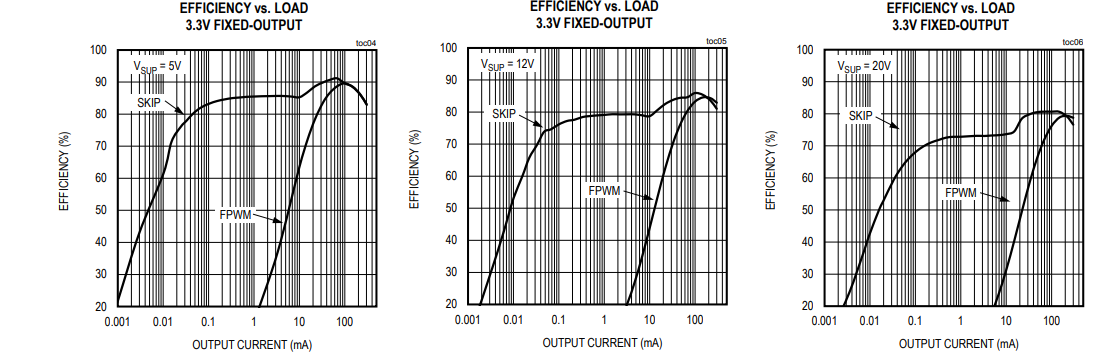
\includegraphics[width=\textwidth]{figures/2_HW_figures/dcdc_efficiency.png}
        \caption{Converter efficiency versus load current at input voltages of \SI{5}{\volt}, \SI{12}{\volt}, and \SI{20}{\volt}, demonstrating performance in both FPWM and skip modes.}
        \label{fig:max77597_efficiency}
    \end{figure}
    

\end{itemize}

\begin{table}[htbp]
    \centering
    \renewcommand{\arraystretch}{1.3}
    \caption{Summary of required voltage rails across PCB subsystems}
    \label{tab:voltage_summary}

    \begin{tabularx}{\textwidth}{|>{\centering\arraybackslash}m{2.5cm}|>{\centering\arraybackslash}m{2cm}|X|X|}
        \hline
        \textbf{Subsystem} &
        \textbf{Voltage} &
        \textbf{Supplied Components} &
        \textbf{Power Source} \\
        \hline

        \textbf{Input Bus}\newline($V_{IN}$) & 
        up to \SI{29.4}{\volt} & 
        DC/DC input,\newline PAC1951 bus ($V_{BUS}$) & 
        External USB Type-C Power Delivery source \\
        \hline

        \textbf{System Logic}\newline($V_{DDS}$) & 
        \SI{3.3}{\volt} & 
        MCU ($V_{DDS}$),\newline PAC1951 ($V_{DD}$),\newline OLED Logic ($V_{DD}$) & 
        DC/DC Converter \\
        \hline

        \textbf{OLED Display}\newline($V_{CC}$) & 
        \SI{7.5}{\volt} & 
        OLED display & 
        SSD1306 internal charge pump \\
        \hline

        \textbf{MCU Internal}\newline($V_{DDR}$) & 
        \SI{1.8}{\volt} & 
        MCU internal RF and Oscillator section& 
        MCU internal DC/DC converter \\
        \hline

        \textbf{MCU Core}\newline($V_{DDC}$) & 
        \SI{1.28}{\volt} & 
        MCU internal digital core & 
        MCU internal Digital LDOs \\
        \hline
        
    \end{tabularx}
\end{table}

The external passive components for the buck converter were sized mathematically following the manufacturer's design guidelines to ensure stability and low noise.

The required inductance ($L$) was calculated to balance the inductor peak-to-peak AC current against the physical size of the component. The value is selected based on the input voltage ($V_{SUP}$), the switching frequency ($f_{SW}$), the expected typical load current ($I_{OUT}$), and a target Inductor Current Ripple Ratio ($LIR$, typically set to $0.3$):

$$L = \frac{V_{OUT} \cdot (V_{SUP} - V_{OUT})}{V_{SUP} \cdot f_{SW} \cdot I_{OUT} \cdot LIR}$$

The output capacitor ($C_{OUT}$) was sized to maintain the output voltage ripple ($V_{RIPPLE(P-P)}$) within the strict limits required by the MCU and ADCs. When utilizing capacitors where the Equivalent Series Resistance ($ESR$) dominates the ripple, the required maximum ESR is calculated as follows:

$$V_{RIPPLE(P-P)} = ESR \cdot I_{LOAD(MAX)} \cdot LIR$$

Finally, the input filter capacitor ($C_{IN}$) was selected to handle the maximum root-mean-square (RMS) ripple current ($I_{RMS}$) drawn by the switching action of the internal MOSFETs. The RMS current requirement reaches its peak when the input voltage is exactly twice the output voltage:

$$I_{RMS} = I_{LOAD(MAX)} \cdot \frac{\sqrt{V_{OUT} \cdot (V_{SUP} - V_{OUT})}}{V_{SUP}}$$

The final implemented circuit is shown in Figure~\ref{fig:max77597_schematic}, where the selected component values are also reported.

An important note must be made regarding the system's ground connections. Proper grounding is critical for the stable, jitter-free operation of the MAX77597 step-down converter. To manage the distinct electrical characteristics within the IC, the device separates its ground into two discrete pins: Analog Ground (AGND) and Power Ground (PGND). The separation of grounds is required to prevent high-frequency switching noise from corrupting the sensitive analog control loops:
\begin{itemize}
    \item \textbf{PGND (Power Ground):} This pin serves as the high-current return path for the internal power MOSFETs and external power components (such as the input capacitor, $C_{IN}$, and output capacitor, $C_{OUT}$). The rapid switching action of the converter generates large current transients (high $di/dt$), which inevitably induce voltage spikes and noise across the power ground plane.
    \item \textbf{AGND (Analog Ground):} This pin acts as the clean, quiet reference ground for the internal analog circuitry, including the \SI{5}{\volt} BIAS regulator, error amplifiers, and feedback comparators. If noisy PGND currents were allowed to flow through the AGND path, it would introduce significant jitter, degrade voltage regulation accuracy, and potentially cause erratic switching behavior.
\end{itemize}


\begin{figure}[htbp]
    \centering
    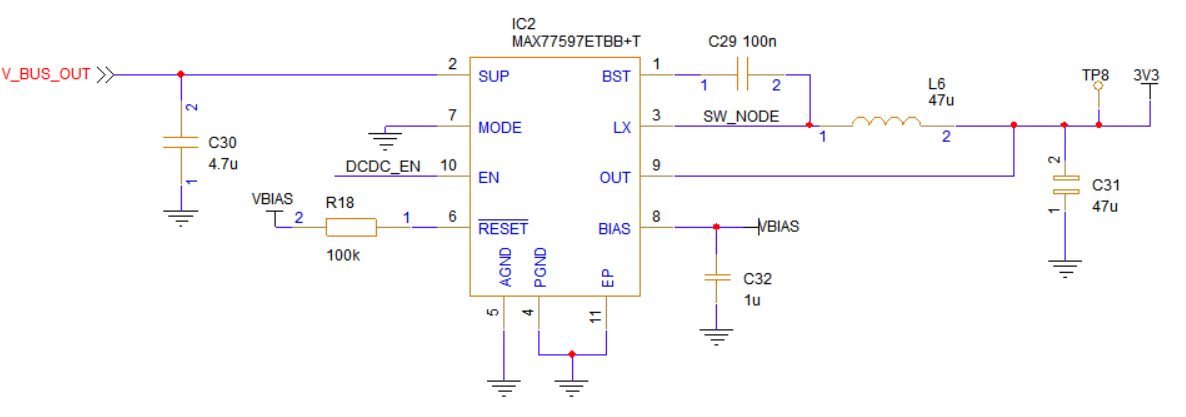
\includegraphics[width=\textwidth]{figures/2_HW_figures/max77597_circuit.png}
    \caption{Schematic diagram of the MAX77597 step-down converter subsystem.}
    \label{fig:max77597_schematic}
\end{figure}

%========================================================
% Connectors - USB Type-C
%========================================================
\newpage
\subsection{Connectors - USB Type-C}

\begin{figure}[H]
    \centering
    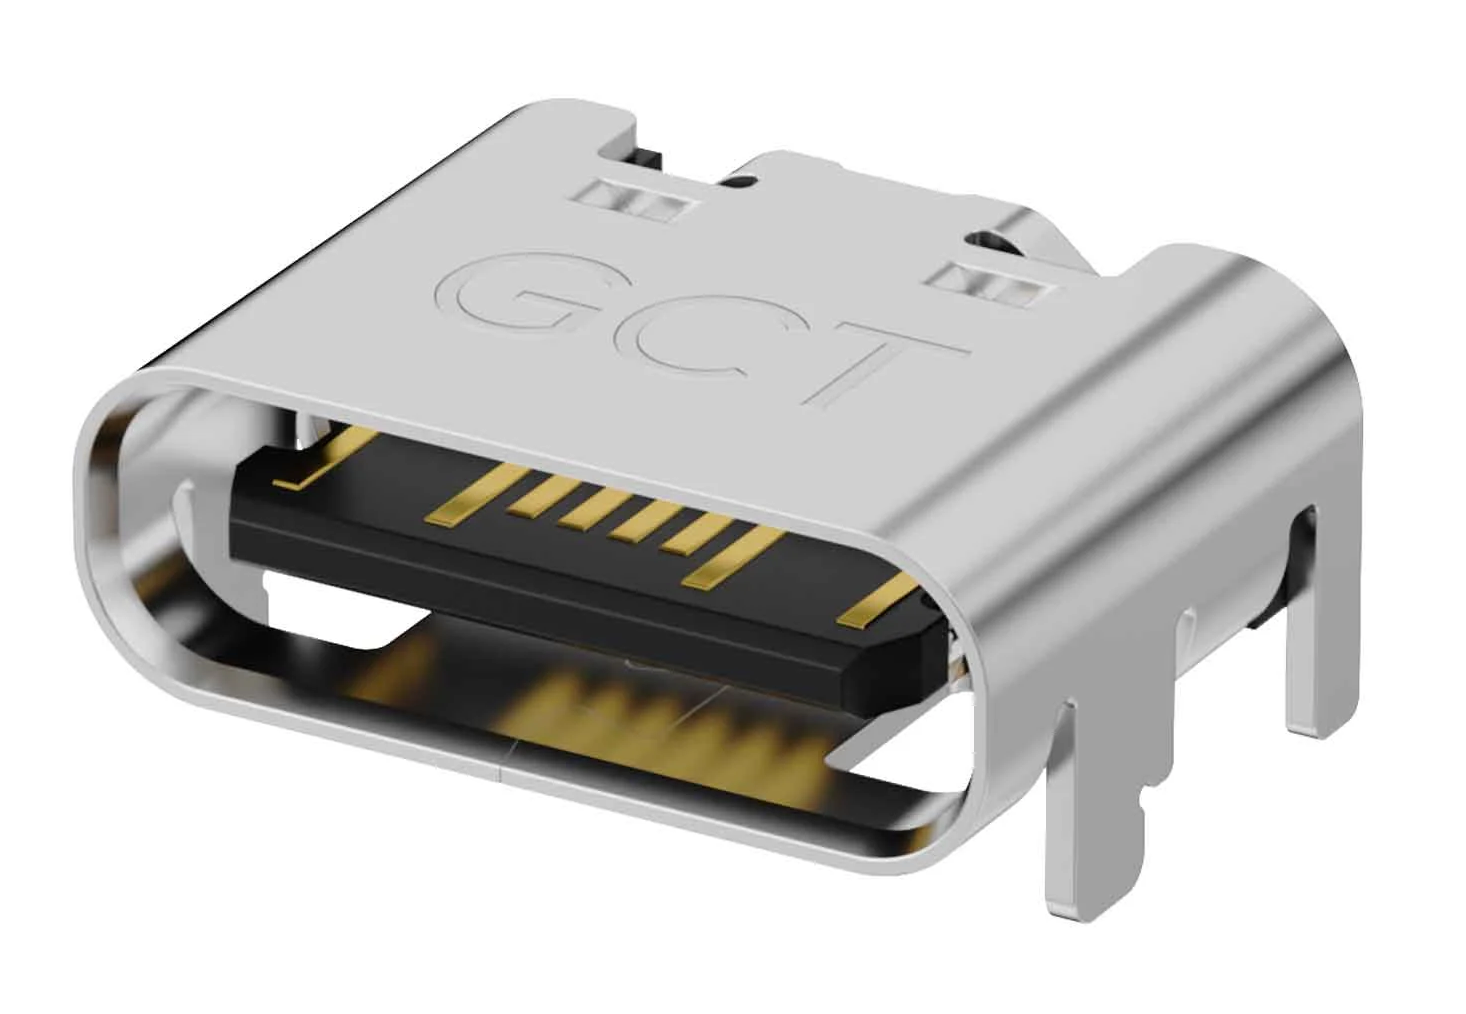
\includegraphics[width=0.4\textwidth]{figures/2_HW_figures/usb.png}
    \caption{USB Type C 16 pin receptacle, SMT horizontal top mount.}
    \label{fig:usb}
\end{figure}

\subsubsection{Component Selection and Requirements Addressed}
The system must operate inline between a power source and a load without interrupting power delivery, while safely handling the full USB Power Delivery 3.1 profile up to \SI{28}{\volt} and \SI{5}{\ampere} (Requirements~\ref{req:volt_table},~\ref{req:curr_rating}, and~\ref{req:inline_op}). To fulfill these physical interface requirements, the GCT USB4215 USB Type-C receptacle was selected for both the input and output ports of the analyzer. The most relevant features that motivated this choice are summarized below:

\begin{itemize}

    \item \textbf{Electrical and Mechanical Characteristics:}

    \begin{table}[H]
        \centering
        \renewcommand{\arraystretch}{1.3}
        \caption{Electrical and mechanical characteristics of the GCT USB4215 receptacle}
        \label{tab:usb4215_characteristics}

        \begin{tabularx}{0.9\textwidth}{|l|X|c|c|c|}
            \hline
            \textbf{Symbol} &
            \textbf{Parameters} &
            \textbf{Typical} &
            \textbf{Maximum} &
            \textbf{Unit} \\
            \hline

            $V_{RATING}$ & Maximum DC voltage rating & - & 48 & \SI{}{\volt} \\
            \hline
            
            $I_{VBUS}$ & Collective current rating for VBUS pins & - & 5.0 & \SI{}{\ampere} \\
            \hline

            $I_{GND}$ & Collective current rating for GND pins & - & 6.25 & \SI{}{\ampere} \\
            \hline

            $R_{CONTACT}$ & Initial contact resistance & - & 40 & \SI{}{\milli\ohm} \\
            \hline
            
            $Cycles$ & Mating durability & 20000 & - & Cycles \\
            \hline

        \end{tabularx}
    \end{table}

    \item \textbf{Extended Power Ratings:} 
    The USB4215 connector is rated for a maximum voltage of \SI{48}{\volt} DC and a collective VBUS current of \SI{5.0}{\ampere}, enabling it to handle up to \SI{240}{\watt} of power. This provides a substantial safety margin for the system's \SI{140}{\watt} target, fully complying with the power delivery requirements (Requirements~\ref{req:volt_table},~\ref{req:curr_rating}, and~\ref{req:pow_rating}).

    \item \textbf{Optimized 16-Pin Configuration:} 
    The receptacle utilizes a 16-pin layout that omits the high-speed SuperSpeed (Tx/Rx) data pins, which are unnecessary for this power analysis application. However, it retains the essential VBUS, GND and Configuration Channel (CC1/CC2) pins. This ensures that the system does not interfere with the USB Power Delivery negotiation process between the source and the sink (Requirement~\ref{req:inline_pd}) while significantly simplifying the PCB layout and assembly.

    \item \textbf{High Durability and Low Contact Resistance:} 
    The connector features an initial contact resistance of just \SI{40}{\milli\ohm} (maximum) and is rated for \num{20000} mating cycles. This minimizes parasitic voltage drops across the inline connection—crucial for maintaining measurement accuracy (Requirement~\ref{req:volt_acc})—and ensures long-term mechanical reliability.

    

\end{itemize}

\subsubsection{Component Sizing and Implementation Details}
To satisfy the inline operation requirement (Requirement~\ref{req:inline_op}), two USB4215 connectors are mounted on opposite edges of the PCB. One acts as the power input from the source, and the other acts as the output to the load. The Configuration Channel (CC1, CC2) are passed straight through between the two connectors. This passive passthrough guarantees that the system remains transparent to the USB Power Delivery negotiation process.

While connectors do not require mathematical sizing in the same way as active power converters, evaluating the worst-case power dissipation ($P_{LOSS}$) across the connector is critical to ensure thermal stability under continuous heavy loads. The maximum power dissipated by the connector's contact resistance ($R_{CONTACT}$) at the absolute maximum rated current ($I_{MAX}$) is calculated as:

$$P_{LOSS} = I_{MAX}^2 \cdot R_{CONTACT}$$

For the maximum targeted operating current of \SI{5}{\ampere} and the worst-case initial contact resistance of \SI{40}{\milli\ohm}, the expected power loss is:

$$P_{LOSS} = (\SI{5}{\ampere})^2 \cdot \SI{40}{\milli\ohm} = \SI{1.0}{\watt}$$

This \SI{1.0}{\watt} worst-case dissipation per connector highlights the necessity of the large VBUS and GND copper pours on the PCB, that will be further analyzed in the layout consideration Section~\ref{layout_considerations}. These pours act not only as high-current carrying traces but also as essential thermal heatsinks to wick heat away from the connector's Surface Mount Technology (SMT) pads, ensuring the system operates safely within the targeted temperature bounds.


%========================================================
%========================================================
%========================================================
% PCB Design
%========================================================
%========================================================
%========================================================
\newpage
\section{PCB Design}


\subsection{Component Placement Strategy}\label{component_placement_strategy}
The physical floorplanning of the PCB was dictated by the need to isolate distinct electrical domains, specifically separating high current power delivery, sensitive analog measurements, noisy switching regulators, and high frequency RF transmission. 

The two USB Type-C connectors are placed on opposite edges of the board to facilitate an intuitive inline connection between the power source and the load. The high-current power path, including the series shunt resistor, the PAC1951 measurement IC, and the MAX77597 step-down converter, is strictly confined to the upper half of the board. 

The CC2640R2F microcontroller (MCU) and the remaining subsystems, such as the user-interface buttons and OLED display connector, are centrally located. This centralized placement is strategic since it minimizes trace lengths and prevents signals from requiring long, convoluted paths with excessive via transitions, thereby improving overall signal integrity. Furthermore, this positions the display and buttons optimally for ergonomic user access and visibility.

Finally, the \SI{2.4}{\giga\hertz} RF matching network and PCB antenna are positioned at the very bottom edge of the PCB. This strict physical separation maximizes the distance from the DC/DC converter in the upper half, effectively preventing high-frequency switching noise from coupling into the sensitive RF front-end.

\begin{figure}[H]
    \centering

    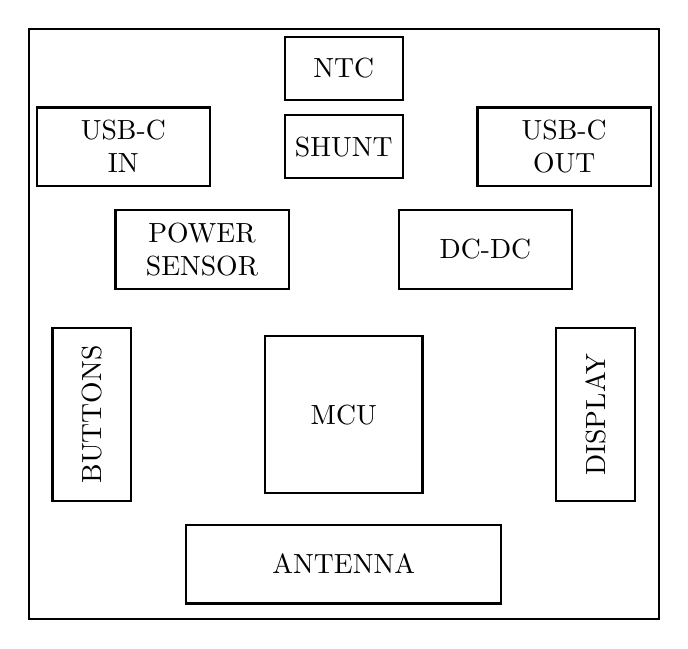
\begin{tikzpicture}[
        block/.style={draw, thick, minimum width=2.2cm, minimum height=1cm, align=center},
        smallblock/.style={draw, thick, minimum width=1.5cm, minimum height=0.8cm, align=center},
        wideblock/.style={draw, thick, minimum width=4cm, minimum height=1cm, align=center},
        box/.style={draw, thick, minimum width=2cm, minimum height=2cm, align=center},
        line/.style={thick}
    ]

    % Outer boundary
    \draw[thick] (0,0) rectangle (8,7.5);

    % USB-C IN / OUT
    \node[block] (usbin) at (1.2,6) {USB-C\\IN};
    \node[block] (usbout) at (6.8,6) {USB-C\\OUT};

    % NTC
    \node[smallblock] (ntc) at (4,7) {NTC};

    % SHUNT
    \node[smallblock] (shunt) at (4,6) {SHUNT};

    % DC-DC
    \node[block] (dcdc) at (5.8,4.7) {DC-DC};

    % Power sensor
    \node[block] (ps) at (2.2,4.7) {POWER\\SENSOR};

    % MCU
    \node[box] (mcu) at (4,2.6) {MCU};

    % Buttons
    \node[block, rotate=90] (buttons) at (0.8,2.6) {BUTTONS};

    % Display
    \node[block, rotate=90] (display) at (7.2,2.6) {DISPLAY};

    % Antenna
    \node[wideblock] (antenna) at (4,0.7) {ANTENNA};


    \end{tikzpicture}

    \caption{System architecture floorplanning.}
    \label{fig:block_diagram}
\end{figure}


%========================================================
% Layer Stackup and Impedance Control
%========================================================
\subsection{Layer Stackup and Impedance Control}\label{stackup}

\subsubsection{Layer Stackup Architecture}
To satisfy the conflicting demands of high-current power delivery (\textbf{Requirement~\ref{req:curr_rating}}), sensitive analog measurements, and high-frequency RF transmission (\textbf{Requirement~\ref{req:ble_tx}}), a 4-layer Printed Circuit Board (PCB) architecture was selected. The chosen stackup (see Figure) provides the necessary routing flexibility and solid reference planes required for a mixed-signal design. 

The layer assignment was strategically defined as follows:
\begin{itemize}
    \item \textbf{Top Layer (L1 - Signal / RF / GND):} Houses all surface-mount components, the \SI{2.4}{\giga\hertz} PCB antenna, the critical RF matching network, and the massive copper polygon pours required to carry the \SI{5}{\ampere} VBUS current. The remaining available area is filled with a ground pour, stitched to the internal and bottom ground planes through a dense via network, providing a low-impedance return path, improved EMI performance, enhanced RF behavior, and effective current return routing.
    \item \textbf{Internal Layer 1 (L2 - Solid GND):} Dedicated entirely as a continuous, unbroken Ground plane. This serves three critical functions: it provides a low impedance return path for all signals, acts as the immediate dielectric reference plane for the RF impedance control, and serves as a massive thermal heat spreader for the power connectors and shunt resistor.
    \item \textbf{Internal Layer 2 (L3 - Power):} Dedicated to the distribution of the internally generated \SI{3.3}{\volt} logic supply ($V_{DDS}$). Using a solid power plane minimizes the power distribution network impedance, improves supply voltage stability, and provides additional inter-plane capacitance with the adjacent ground layer, contributing to high-frequency decoupling.
    \item \textbf{Bottom Layer (L4 - Signal / GND):} Used for secondary signal routing and placement of test points required for debugging and validation activities. The remaining area is filled with a ground pour, stitched to the top and internal ground layers through vias.    

\end{itemize}

\begin{figure}[H]
    \centering
    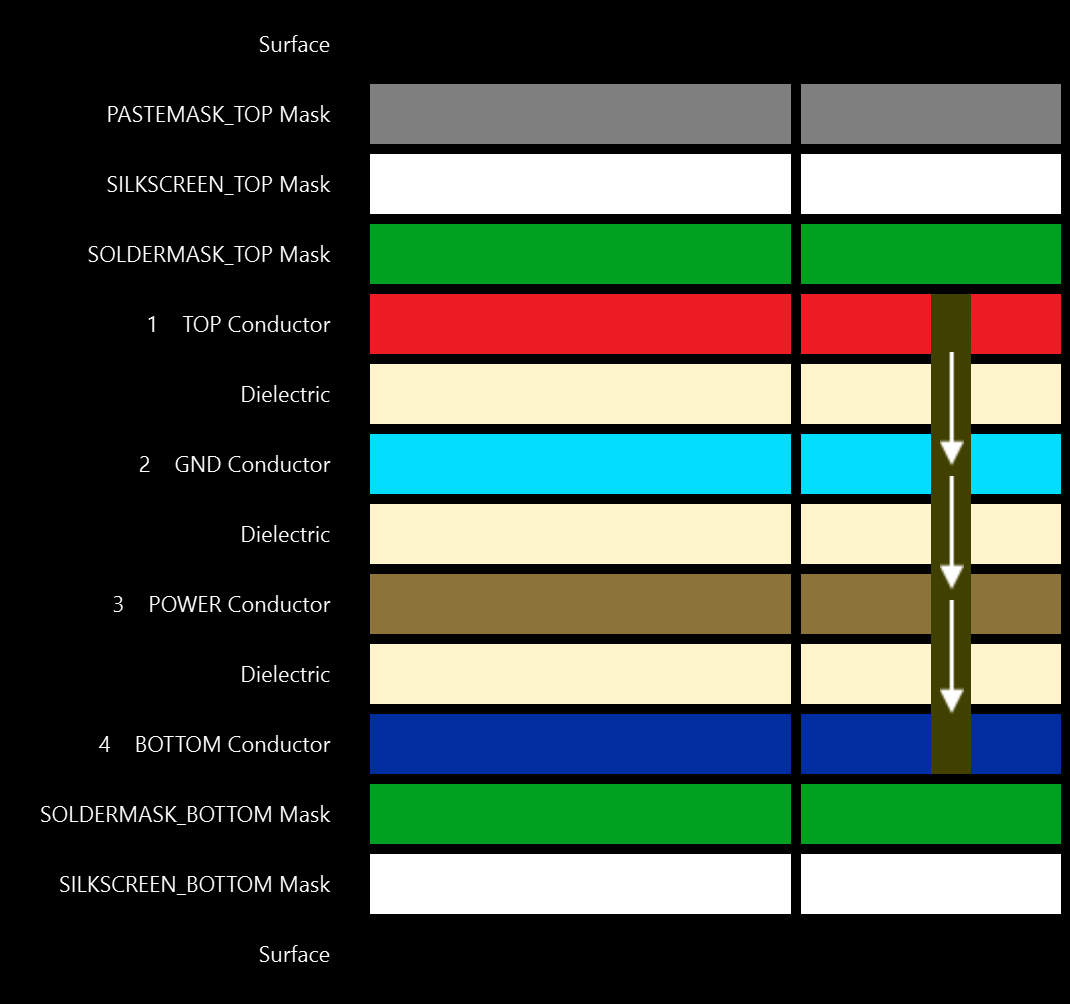
\includegraphics[width=0.75\textwidth]{figures/2_HW_figures/stack_pcb.png}
    \caption{Cross-sectional profile of the 4-layer PCB stackup.}
    \label{fig:layer_stackup}
\end{figure}


\subsubsection{RF Impedance Control}\label{rf_impedance_control}
To ensure reliable BLE communication, the RF front-end must minimize signal reflection and maximize power transfer to the antenna. This dictates that the trace connecting the CC2640R2F microcontroller to the antenna feed point must be designed as a controlled \SI{50}{\ohm} transmission line.

In the PCB manufacturer website, the JLC04161H-7628 stack-up shown in Figure~\ref{fig:impedance_calc} was selected as a cost effective solution that still provides adequate electrical performance for the target application. Given the 4-layer stackup, the RF transmission line is modeled as a surface coplanar waveguide with ground (CPWG). The characteristic impedance $Z_0$ is a function of the trace width $W$, the clearance gap to the adjacent top layer ground pour $S$, the copper thickness $T$, the dielectric constant of the FR-4 substrate ($\epsilon_r \approx 4.5$), and the dielectric height to the reference ground plane $H$. By utilizing the manufacturer's specific tool based on the selected JLC04161H-7628 stackup parameters, the trace width was mathematically calculated to hit the target \SI{50}{\ohm} impedance.

\begin{figure}[H]
    \centering
    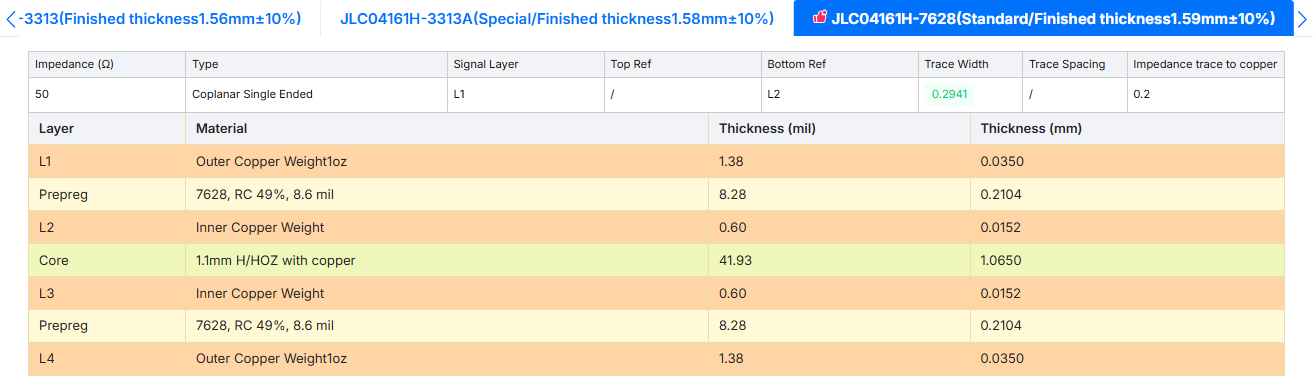
\includegraphics[width=\textwidth]{figures/2_HW_figures/stack_jlc.png}
    \caption{PCB manufacturer's impedance calculation tool used to determine the required \SI{50}{\ohm} trace width, based on the selected layer stack-up and material properties.}
    \label{fig:impedance_calc}
\end{figure}

%========================================================
% Constraints and Design Rules Considerations
%========================================================

\subsection{Constraints and Design Rules Considerations}
The Design Rule Check (DRC) parameters and layout constraints were defined to balance optimal electrical performance with cost effective, standard manufacturing capabilities (\textbf{Requirement~\ref{req:packages}}).

\subsubsection{Trace Width Sizing}
Conductor widths were categorically assigned based on their specific electrical domain:
\begin{itemize}
    \item \textbf{Power Lines (VBUS, GND, \SI{3.3}{\volt}):} As will be later discussed in section~\ref{vbus_size}, the \SI{5}{\ampere} VBUS and GND nets were routed massive multi-layer polygon pours rather than standard traces to prevent thermal overload and excessive voltage drop. The \SI{3.3}{\volt} logic supply, delivering up to \SI{300}{\milli\ampere} from the MAX77597, was routed with minimum trace widths of \SI{0.25}{\milli\meter} to ensure low DC resistance while still allowing routing access through densely populated areas of the PCB.
    \item \textbf{RF Lines (\SI{2.4}{\giga\hertz}):} The antenna feed trace width was derived from controlled impedance requirements rather than an arbitrary design choice. Based on the analysis in Section~\ref{rf_impedance_control}, a CPWG structure was used to achieve a \SI{50}{\ohm} characteristic impedance, resulting in a calculated trace width of \SI{0.294}{\milli\meter}.
    \item \textbf{Analog Lines:} The analog signal traces are routed with minimum width to reduce the exposed copper surface that can couple to external noise sources. Moreover, these traces carry negligible current, making narrow routing fully appropriate from an electrical perspective. Differential traces connecting the PAC1951 to the shunt resistor and the NTC sensing network follow this routing strategy. These traces are implemented with a width of \SI{0.15}{\milli\meter}, also ensuring compliance with the lowest-cost manufacturing class supported by the PCB manufacturer.
    \item \textbf{Normal/Digital Lines (GPIO, $I^2C$):} Similarly to analog traces, GPIO digital lines are low-current signals. In this case, narrow routing is particularly useful to allow escape routing from the dense MCU pin area and to maintain routability in high-density regions of the PCB layout, without compromising signal integrity. These traces are implemented with a width of \SI{0.15}{\milli\meter}.
\end{itemize}

\subsubsection{Via Dimensions}

To reduce manufacturing costs and simplify the PCB fabrication process, only Plated Through-Hole (PTH) vias were used throughout the design. This approach avoids the additional complexity and cost associated with blind, buried, or microvias while remaining fully compatible with the routing density and performance requirements of the system.

The standard via size was set to a \SI{0.3}{\milli\meter} drill diameter with a \SI{0.5}{\milli\meter} annular ring pad. This \SI{0.3}{\milli\meter} via hole size incurs no additional drilling charges, while remaining small enough to be densely arranged in via arrays for thermal dissipation. It also fits within the exposed thermal pads of the ICs without causing solder drainage issues during reflow, ensuring both manufacturability and reliable thermal/electrical performance.

\subsubsection{Component Spacing}
Clearance constraints were dictated by assembly reliability (Requirement~\ref{req:assembly}):
\begin{itemize}
    \item \textbf{Passive to Passive Clearance:} Minimum spacing of \SI{0.5}{\milli\meter} was defined to ensure reliable manual soldering and avoid solder bridging, while still allowing high component density in compact regions of the PCB.
    
    \item \textbf{IC to Passive Clearance:} Increased spacing of \SI{1.5}{\milli\meter} was adopted around integrated circuits to facilitate probe access, improve thermal relief during rework, and reduce the risk of accidental solder bridging in densely routed areas.
    
    Figure~\ref{fig:ic_clearance} shows a representative section of the PCB layout illustrating the implemented IC-to-passive spacing.

    \begin{figure}[H]
        \centering
        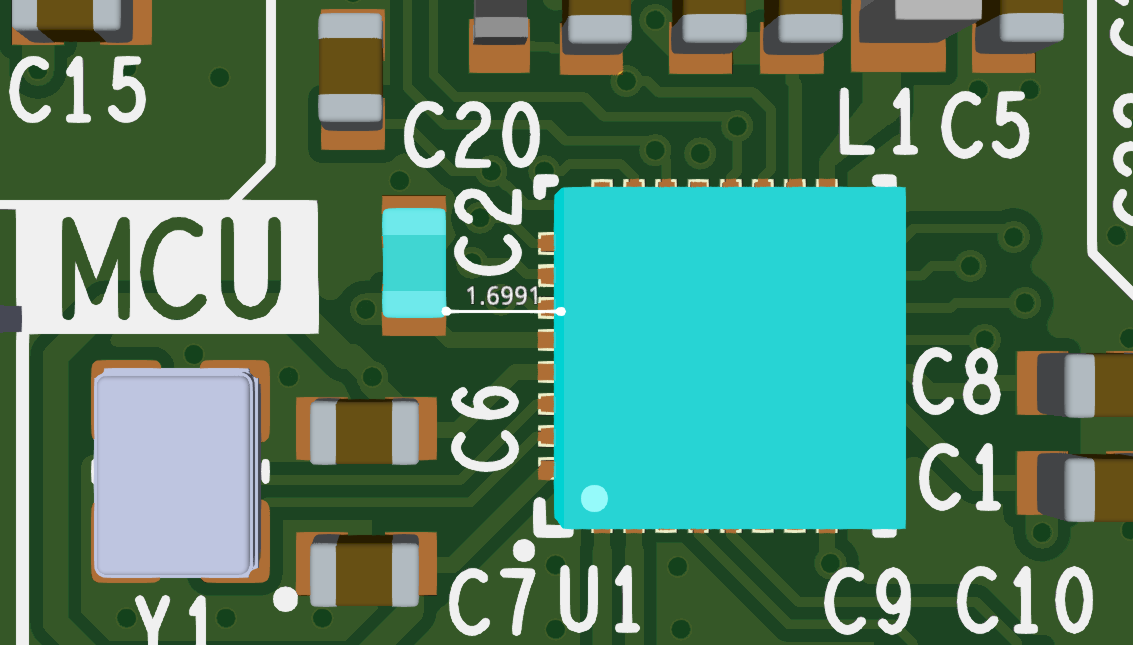
\includegraphics[width=0.7\textwidth]{figures/2_HW_figures/component_clearance.png}
        \caption{Detail of IC to passive clearance measurement on the PCB layout.}
        \label{fig:ic_clearance}
    \end{figure}

\end{itemize}


\subsection{Routing and Layout Considerations}\label{layout_considerations}

    \subsubsection{High-Current Power Path (VBUS)}\label{vbus_size}
        The primary challenge in the power path layout was routing the \SI{5}{\ampere}, \SI{28}{\volt} (up to \SI{140}{\watt}) USB Power Delivery bus between the input and output connectors without exceeding thermal limits or inducing significant voltage drops, which could compromise measurement accuracy (\textbf{Requirement~\ref{req:volt_acc}}). Standard trace routing is insufficient for this current density. 

        To determine the appropriate copper sizing, the Saturn PCB Toolkit was utilized to model the conductor properties, as illustrated in Figure~\ref{fig:saturn_pcb_calc}. Calculations based on a standard \SI{1}{oz/ft^2} (\SI{35}{\micro\meter}) base copper weight demonstrated that a trace width of \SI{4.6}{\milli\meter} carrying \SI{5}{\ampere} yields a safe temperature rise of \SI{20}{\degreeCelsius} (reaching \SI{45}{\degreeCelsius} at a \SI{25}{\degreeCelsius} ambient). Additionally, the predicted voltage drop across this conductor is approximately \SI{16.3}{\milli\volt}.

        To implement this safely and provide additional thermal and electrical margin, \SI{2.8}{\milli\meter} wide copper polygon pours were used to connect the VBUS pins of the USB-C receptacles (see Figure~\ref{fig:main_bus_layout}). By extending these polygons on both the top and bottom layers, the effective cross section exceeds the minimum required width of \SI{4.6}{\milli\meter} when considering parallel conduction paths across multiple layers. To further improve thermal dissipation and current sharing, the same pours are replicated on the internal copper layers and stitched together using dense via arrays. This multi-layer interconnection strategy reduces the overall DC resistance, distributes current more uniformly across the stack-up, and improves heat spreading throughout the PCB structure. The connection of the GND pins is implemented using the same strategy, by exploiting the existing ground planes on layers L1, L2, and L4.

        \begin{figure}[H]
            \centering
            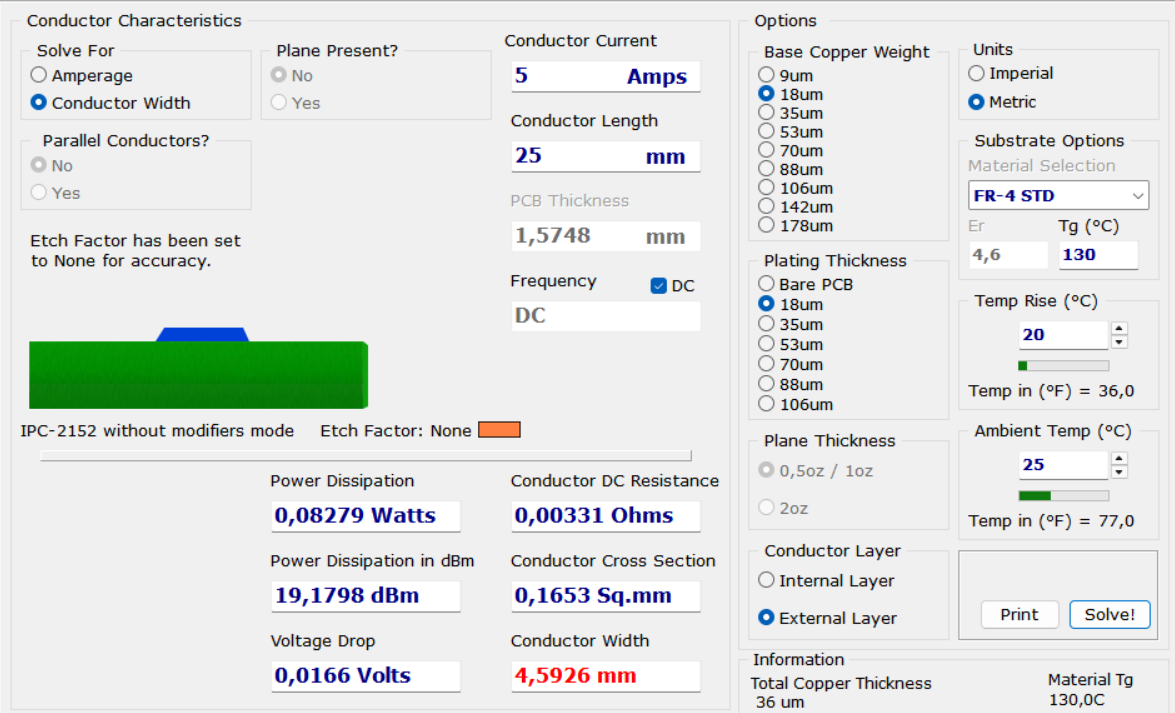
\includegraphics[width=0.9\textwidth]{figures/2_HW_figures/pcb_toolkit.png}
            \caption{Conductor properties calculation using the Saturn PCB Toolkit used to verify trace width.}
            \label{fig:saturn_pcb_calc}
        \end{figure}

        \begin{figure}[H]
            \centering
            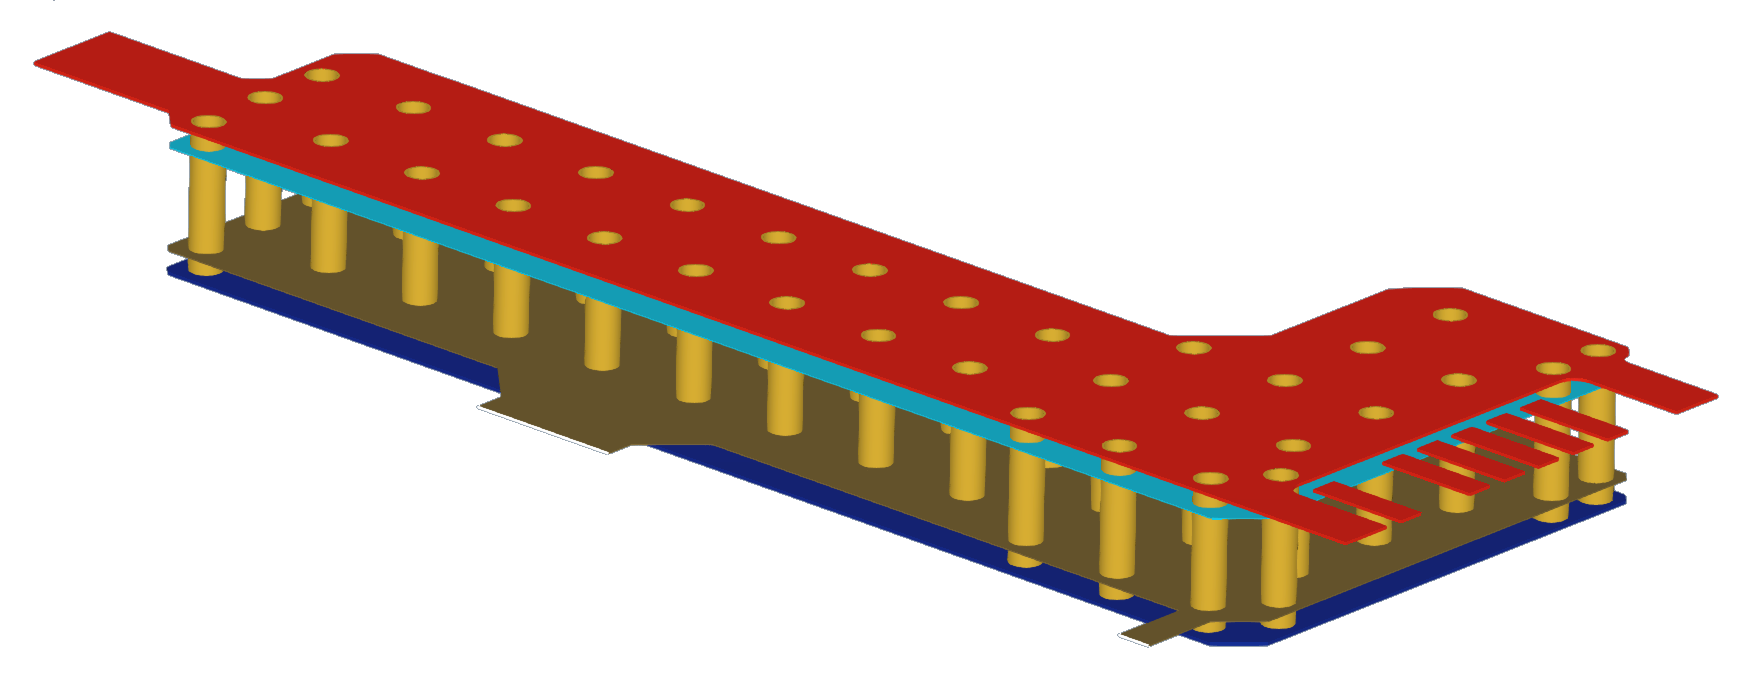
\includegraphics[width=0.9\textwidth]{figures/2_HW_figures/main_bus_section.png}
            \caption{Copper polygon pours and via stitching used for the high-current VBUS.}
            \label{fig:main_bus_layout}
        \end{figure}


        
    \subsubsection{Switching Power Supply (DC/DC)}
    The layout of the MAX77597 step-down converter focuses on minimizing Electromagnetic Interference (EMI) and parasitic ringing. The input capacitor ($C_{IN}$) and output capacitor ($C_{OUT}$) are placed as physically close to the IC pins as possible. This tight placement minimizes the area of the high $di/dt$ switching loops. The inductor is positioned immediately adjacent to the switching node (LX) pin to keep the noisy copper area small, reducing capacitive coupling to nearby analog traces. 

    Furthermore, the layout strictly implements the grounding isolation strategy established during the schematic design phase (see Section~\ref{sec:schematic_max77597}). Because the high-current switching action induces significant voltage transients on the power return path, the Analog Ground (AGND) and Power Ground (PGND) are physically separated on the top layer. The exposed thermal pad (EP) and the returns for the high-current components ($C_{IN}$ and $C_{OUT}$) are tied directly to the main GND plane. Conversely, the sensitive internal \SI{5}{\volt} BIAS regulator capacitor is referenced exclusively to the quiet AGND pin using an isolated trace. To prevent ground loops while establishing a common system reference, these two distinct ground domains are tied together at a single point, forming a star-ground topology. The star point is located directly at the negative thermal pad of the IC, as recommended in the device datasheet~\cite{max77597_datasheet} and illustrated in Figure~\ref{fig:dcdc_layout}. This approach minimizes ground-loop currents, reduces coupling between noisy and sensitive return paths, and ensures a controlled reference potential for the entire system.

    \begin{figure}[H]
    \centering
        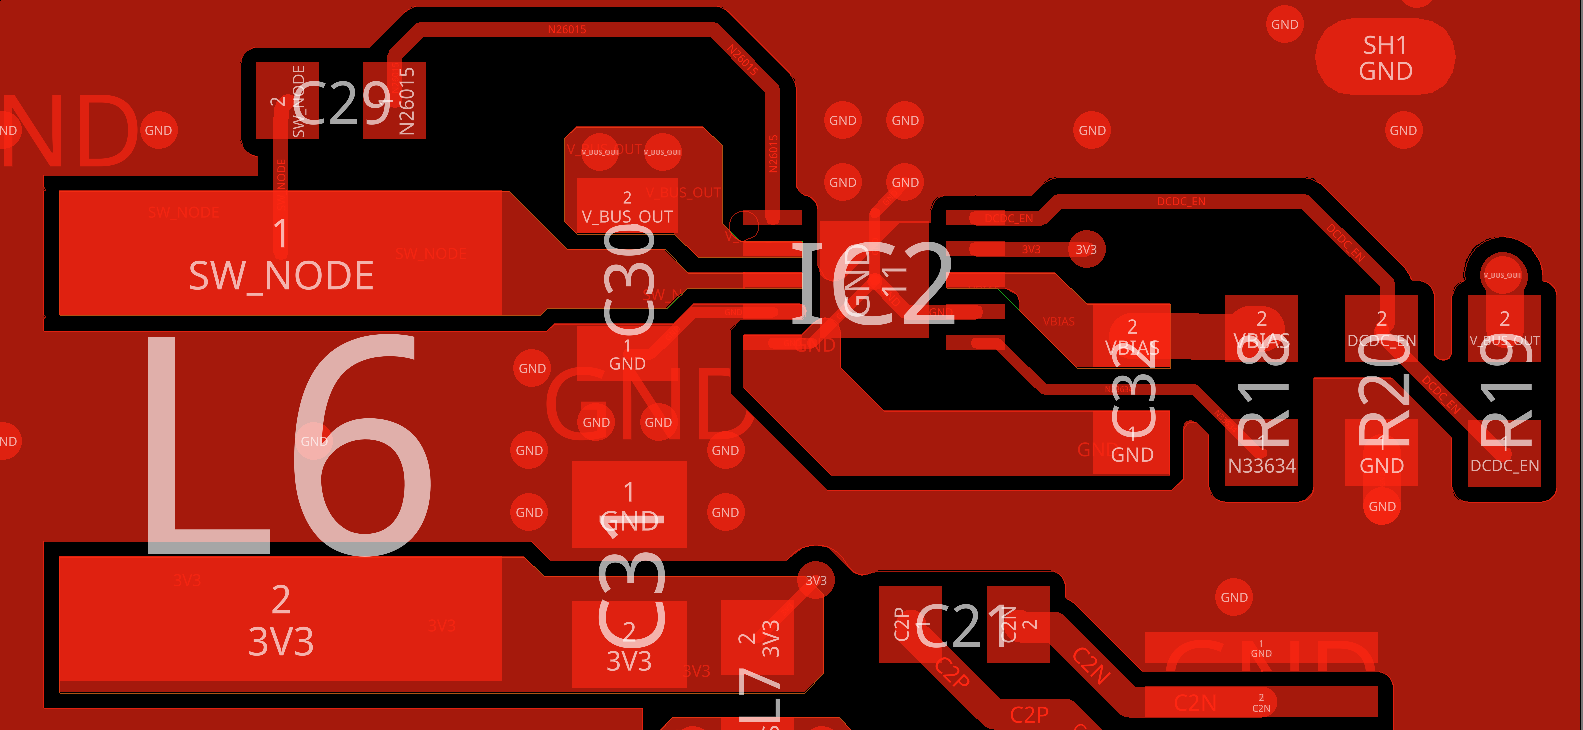
\includegraphics[width=0.9\textwidth]{figures/2_HW_figures/dcdc_layout.png}
        \caption{PCB layout of the MAX77597 step-down converter.}
        \label{fig:dcdc_layout}
    \end{figure}


    \subsubsection{RF Matching Network and Antenna}
    As established in the component placement strategy section \ref{component_placement_strategy}, the IFA antenna and its matching network are strategically positioned at the edge of the PCB to maximize their physical separation from the high-frequency switching noise generated by the DC/DC converter. This placement also creates a dedicated area free from sensitive circuitry, reducing the risk of RF noise coupling.

    The \SI{2.4}{\giga\hertz} Bluetooth transmission requires meticulous impedance control to ensure maximum power transfer and minimal signal reflection. The trace connecting the MCU RF pins to the PCB antenna is routed as a controlled \SI{50}{\ohm} impedance line using a Coplanar Waveguide with Ground (CPWG) structure. To isolate this sensitive transmission line from internal board noise and prevent electromagnetic leakage, a layout technique known as "via fencing" was applied. As shown in Figure~\ref{fig:rf_layout}, the top-layer ground pours flanking the RF trace are heavily populated with a continuous row of vias connecting directly to the solid internal L2 ground plane. This creates a protective electromagnetic boundary, functioning similarly to a coaxial cable embedded within the PCB.

    Additionally, the passive components comprising the impedance matching network are placed in a tightly packed geometry directly between the MCU and the antenna feed point. This minimizes any uncalculated parasitic inductance or capacitance that could detune the network. Finally, to allow the antenna to radiate efficiently into free space, "keep-out" zones were created. The PCB area directly beneath and immediately surrounding the antenna is entirely devoid of copper on all layers (Top, In1, In2, and Bottom) to prevent signal absorption and impedance mismatch. For the same reason, the components placed in close proximity to the antenna section ($S2$ and $J4$) are intended exclusively for testing and debugging purposes. These components are included to facilitate testing and validation during the development phase. In the final product, they will not be populated, thereby increasing the clearance area around the antenna and further reducing undesired degradation of the transmitted signal.

    \begin{figure}[htbp]
        \centering
        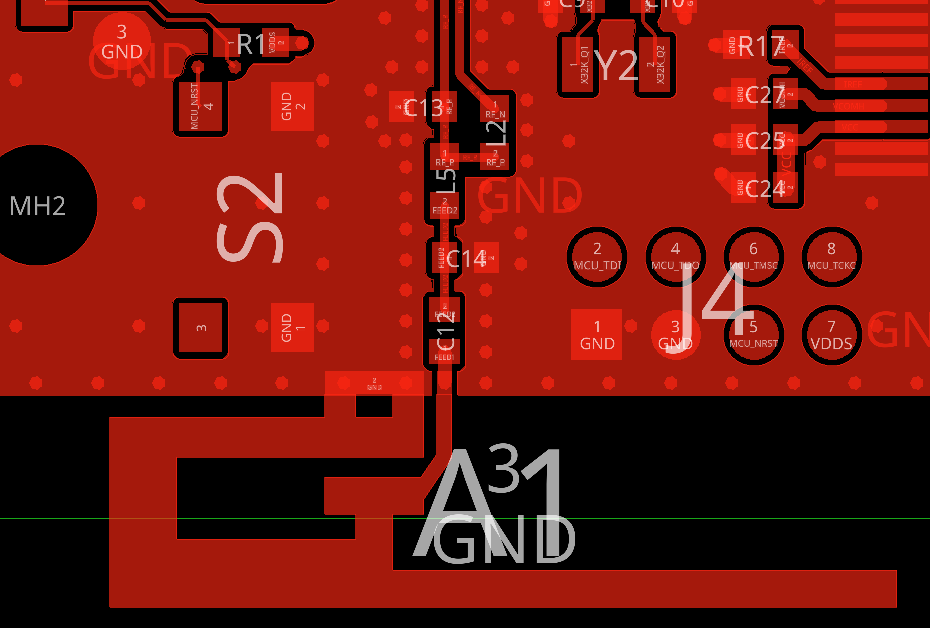
\includegraphics[width=0.9\textwidth]{figures/2_HW_figures/rf_layout.png}
        \caption{PCB layout of the RF subsystem, illustrating the tightly grouped matching network, the via fencing and the copper keep-out zone surrounding the antenna.}
        \label{fig:rf_layout}
    \end{figure}


    \subsubsection{Precision Analog Measurement}
    Accurate power measurement relies heavily on the layout of the PAC1951 and its associated \SI{10}{\milli\ohm} shunt resistor. To ensure that current measurement noise is minimized, the sense traces connecting the shunt resistor to the PAC1951 inputs are routed using the Kelvin connection terminals, available on the $R10$ package. These traces are tapped directly from the inner edges of the resistor pads to bypass the voltage drop introduced by high-current solder joints. Furthermore, the sense lines are routed as a tightly coupled differential pair and the PAC1951 input differential filter is placed with a symmetrical layout to minimize any mismatch between the two sensing paths.

    Figure~\ref{fig:kelvin_connection} illustrates the implemented Kelvin sensing layout used in the design.

    \begin{figure}[H]
        \centering
        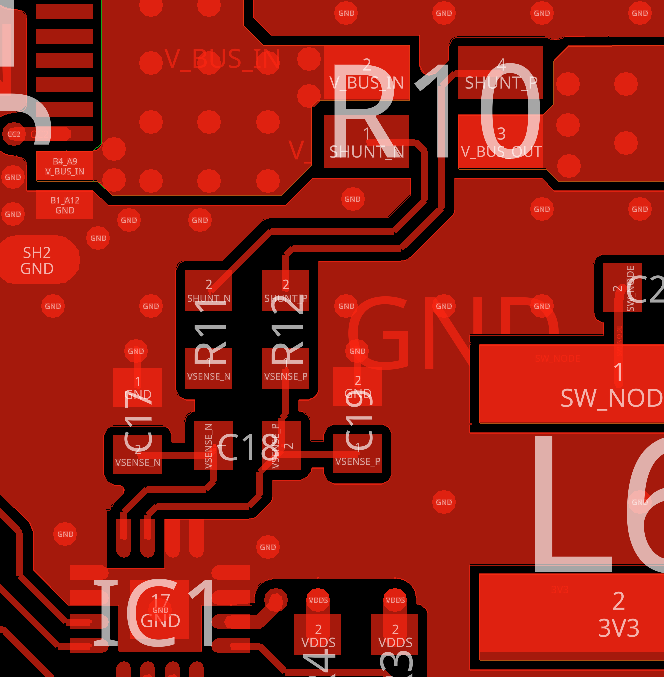
\includegraphics[width=0.65\textwidth]{figures/2_HW_figures/kelvin_connection.png}
        \caption{Kelvin connection layout of the $R10$ shunt resistor and PAC1951 sensing inputs.}
        \label{fig:kelvin_connection}
    \end{figure}


\subsubsection{Display Placement}

The physical placement and routing of the display required careful mechanical consideration to maximize usable board space while maintaining an ergonomic user interface. Rather than placing the bulky display on the already densely populated top layer, the flexible connector was strategically mounted on the right side of the board, in order for the display to be bent towards the back side of the pcb, where no SMD components are mounted, as shown in Figure~\ref{fig:display_placement}. To avoid increasing the overall PCB length and to eliminate the need for rerouting to accommodate additional clearance, the display module is placed in close proximity to the TH JTAG programming connector. This arrangement does not create any functional issues because, during the development and testing phase, the display is intentionally left non folded in its final position, allowing simultaneous access to the programming connector and full visibility of the display. In the final product, the JTAG connector is not populated leaving sufficient space for the display to be permanently attached on the back side of the board.

Mechanically, the flexible flat cable of the OLED display is routed around the edge of the PCB to connect the display module mounted on the opposite side of the assembly. To protect the delicate flexible connection from excessive bending stress and potential damage, a rounded-edge cutout is incorporated into the PCB directly beneath the cable path, allowing the cable to remain within the overall PCB outline.

\begin{figure}[H]
    \centering
    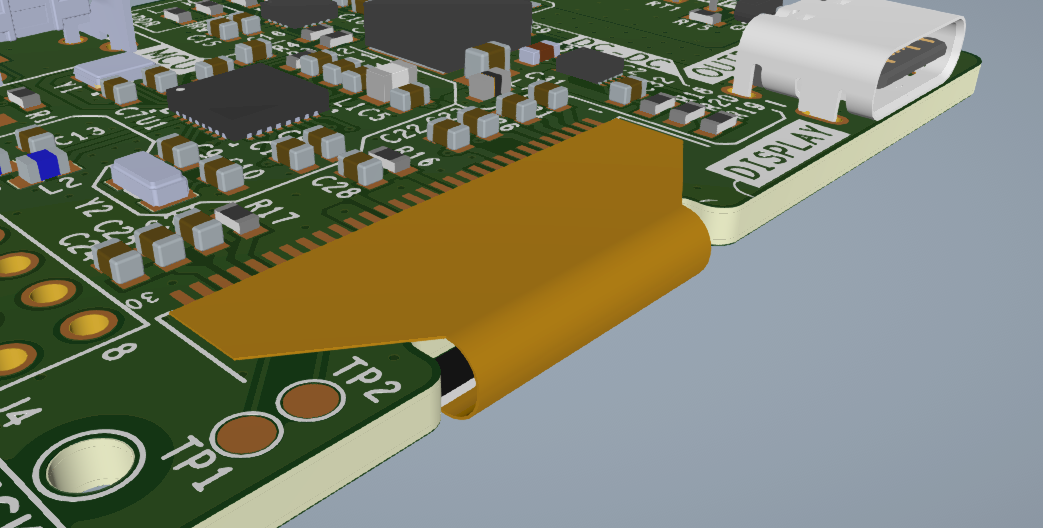
\includegraphics[width=0.8\textwidth]{figures/2_HW_figures/3d_display_top.png}
    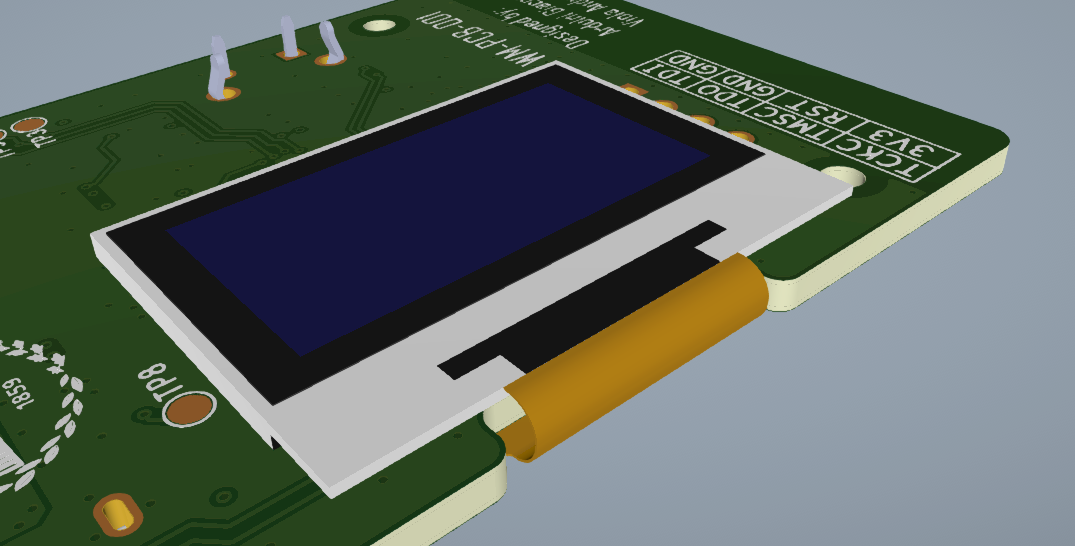
\includegraphics[width=0.8\textwidth]{figures/2_HW_figures/3d_display_bottom.png}
    \caption{Display connector placement and routing strategy showing the display folding towards the back side of the PCB.}
    \label{fig:display_placement}
\end{figure}


\subsubsection{Grounding Strategy}

Via usage in the PCB layout follows a hierarchical strategy, starting from local component-level optimization and extending to global plane interconnection across the 4-layer stack-up introduced in Section~\ref{stackup}.

At the local level, vias are placed in close proximity to high-speed and sensitive components (see Figure~\ref{fig:local_via_decoupling}). This includes ground vias adjacent to IC power pins, decoupling capacitors, and mixed-signal devices. The primary objective of this placement is to minimize current loop areas, reduce parasitic inductance, and improve high-frequency decoupling effectiveness.

In addition to local grounding, a broader via stitching strategy is applied across the entire PCB (see Figure~\ref{fig:via_stitching_detail}). This technique interconnects the copper planes defined in the 4-layer stack-up, ensuring a continuous low-impedance path between ground and power domains. From a thermal perspective, via arrays provide vertical heat conduction paths that improve heat spreading across the PCB thickness, reducing localized hot spots in high-current regions such as VBUS and GND distribution networks. From an electrical perspective, via stitching reduces ground impedance and minimizes inductive discontinuities between layers. This is particularly important for high-frequency switching currents and RF-sensitive sections, where uncontrolled return paths can lead to electromagnetic interference and degraded performance.

\begin{figure}[H]
    \centering
    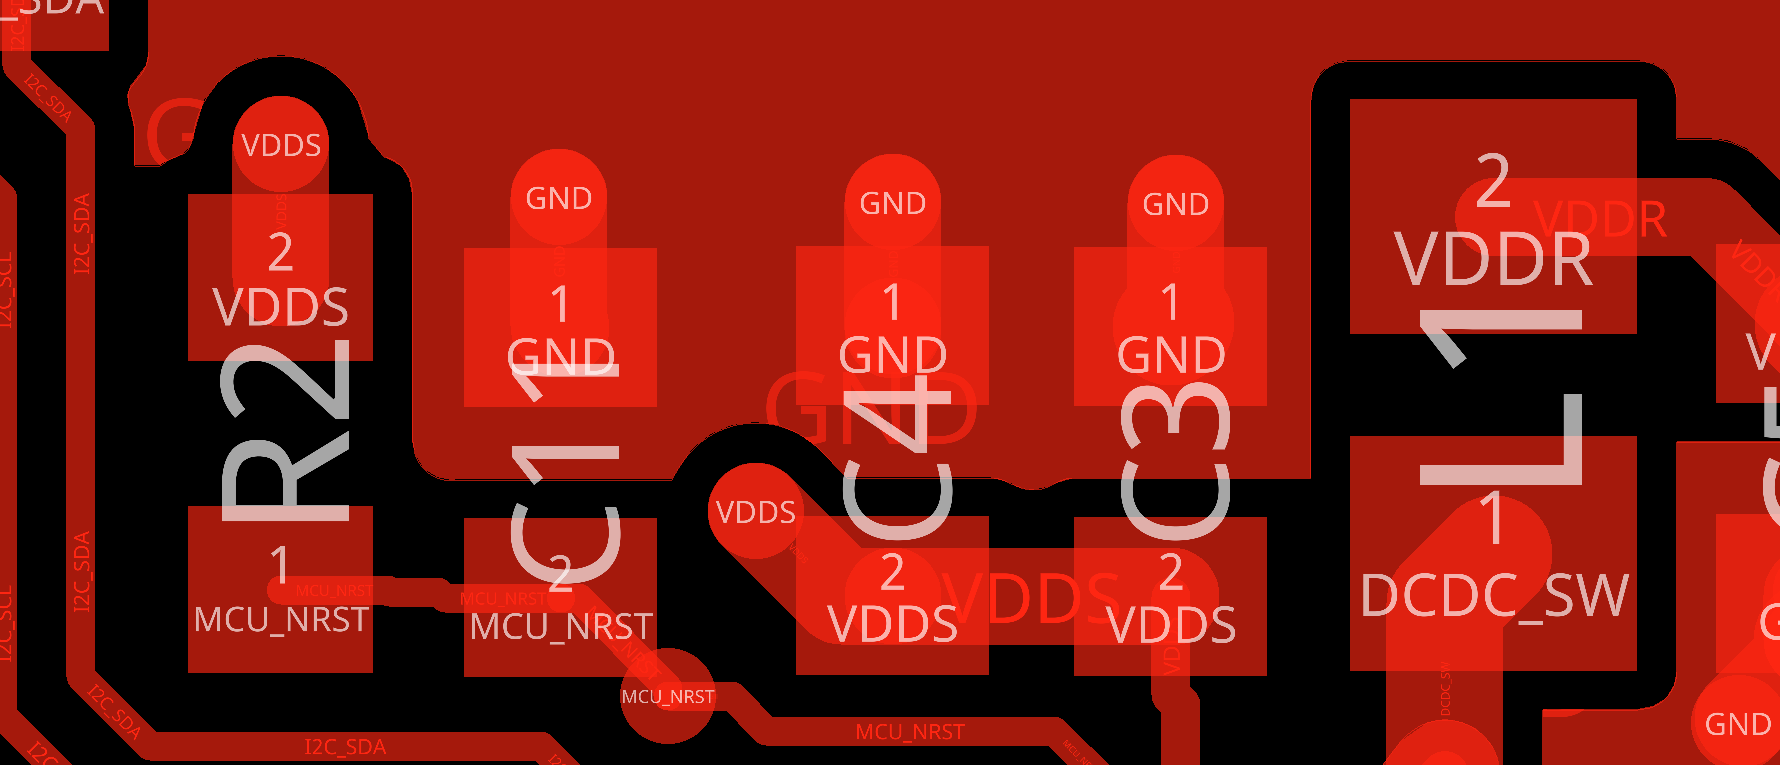
\includegraphics[width=0.75\textwidth]{figures/2_HW_figures/local_via_decoupling.png}
    \caption{Local placement of ground vias near IC power pins and decoupling capacitors to minimize loop inductance and improve high-frequency decoupling performance.}
    \label{fig:local_via_decoupling}
\end{figure}

\begin{figure}[H]
    \centering
    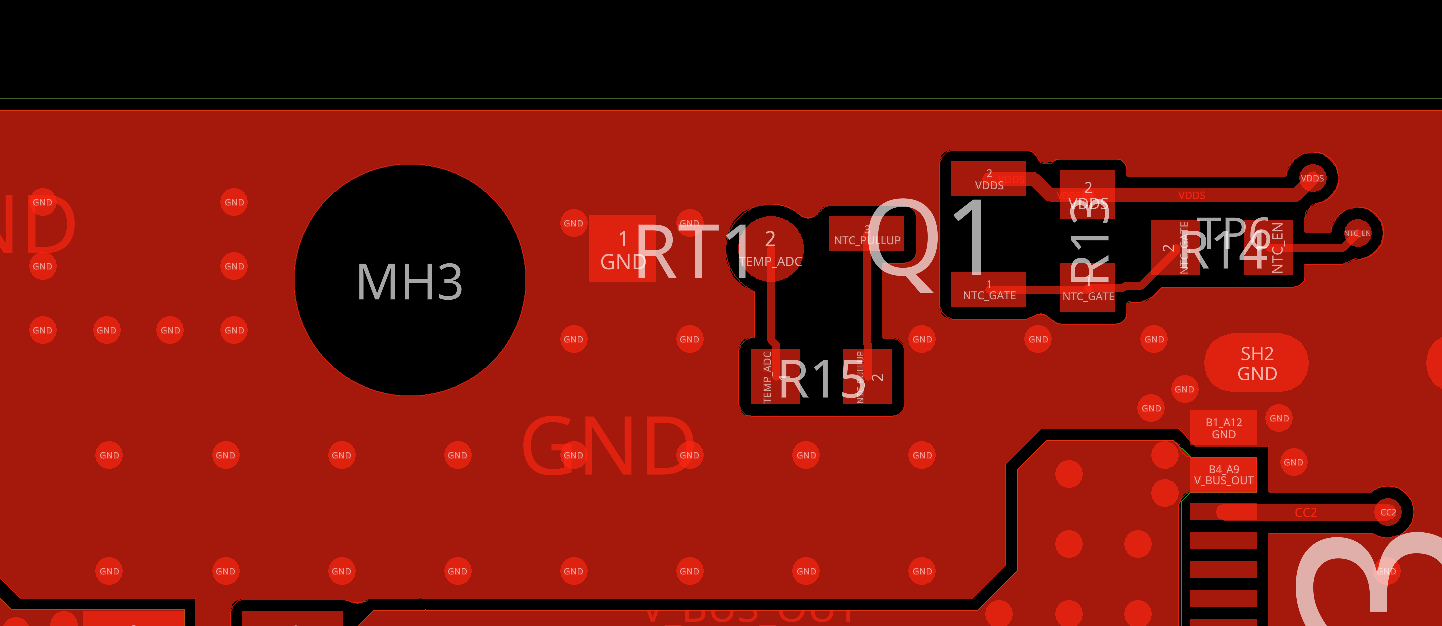
\includegraphics[width=0.85\textwidth]{figures/2_HW_figures/via_stitching_detail.png}
    \caption{Detail of the global via stitching strategy used to interconnect ground planes across the 4-layer stack-up.}
    \label{fig:via_stitching_detail}
\end{figure}



